ParMA support for balancing 2D and 3D unstructured meshes with complex
topological features are demonstrated in the following subsections.
First, we compare ParMA against its predecessor LIIPBMod on up to 256Ki
(256*2$^{10}$) parts.
We then test the effect of ParMA's entity selection features described
in Section~\ref{sec:entSelection} on partition quality and imbalance.
Then, we present ParMA's ability to improve partitions created with graph and
geometric partitioning methods on up to 1Mi ($2^{20}$) parts.
Lastly, we discuss the effect of partition improvement on the scalability of
PHASTA computational fluid dynamics.

\subsection{LIIPBMod Comparison} \label{sec:liipbmodComparison}

We compare the performance of ParMA vertex$>$element improvement against
LIIPBMod on a 64Ki, 128Ki, and 256Ki partition of a 941 million element
tetrahedral abdominal aortic aneurysm (AAA) mesh.
This mesh was generated by successively refining the initial coarse mesh shown
in Fig.~\ref{fig:AAA}.
Three test partitions of the mesh were created by running local ParMETIS (one
instance per process~\cite{Zhou2010}) part k-way on a 16Ki base partition
created with global ParMETIS part k-way.
Our partition improvement test then executed ParMA and LIIPBMod on the three
partitions using the Mira Blue Gene/Q system at the Argonne
Leadership Computing Facility (ALCF).

Fig.~\ref{fig:liipbmod-v-parma} depicts the change in vertex and element
imbalance resulting from ParMA and LIIPBMod.
In these tests LIIPBMod targets a 5\% vertex imbalance and ParMA targets 5\%
vertex and element imbalance.
Note that LIIPBMod does not explicitly target reducing the
element imbalance; it simply tries not to harm it significantly while balancing
vertices.
LIIPBMod balancing stagnates at around 10\% for the vertex imbalance and, at
256Ki, increases the element imbalance by two percentage points.
At all three partition sizes ParMA meets the vertex and element imbalance target
of 5\% and executes 75\% faster than LIIPBMod.
For these partitions ParMA and LIIPBMod have an insignificant effect (less than
one percent) on the total number of vertices.
The ParMA features that support fast balancing are discussed in
Sections~\ref{sec:parma},~\ref{sec:targeting}, and~\ref{sec:entSelection}.
Next, we discuss the performance cost and partition quality improvements
of these features.

\begin{figure} \centering
  \includegraphics[width=.6\textwidth]{results/liipbmod-v-parma/aaa-a1m2/modelAnd1pt8MelmMesh.eps}
  \caption{
    Abdominal aortic aneurysm (AAA) geometric model and close-up view of a coarse mesh.
  }
  \label{fig:AAA}
\end{figure}

\begin{figure} \centering
  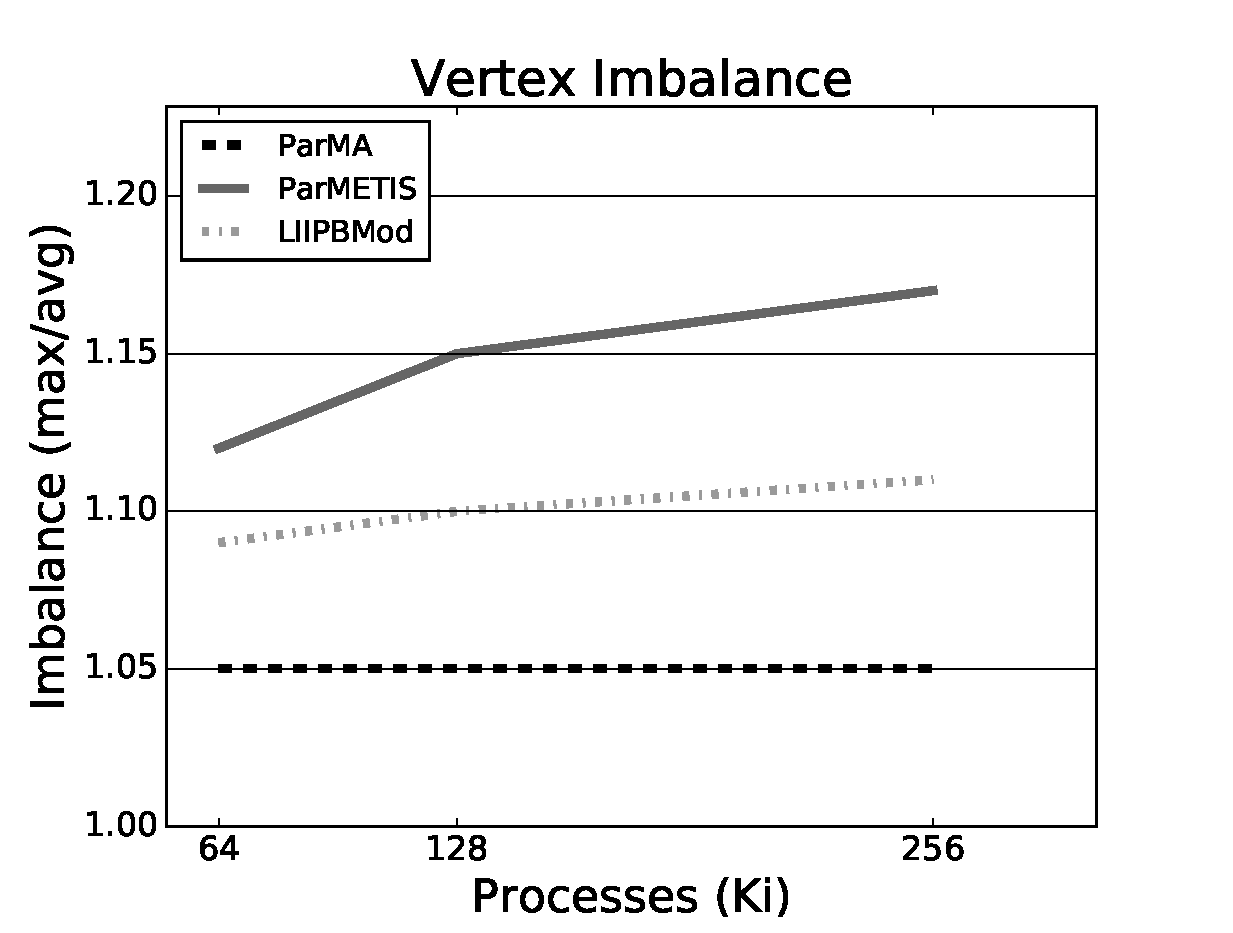
\includegraphics[width=.6\textwidth]{results/liipbmod-v-parma/vtxImb.eps}
  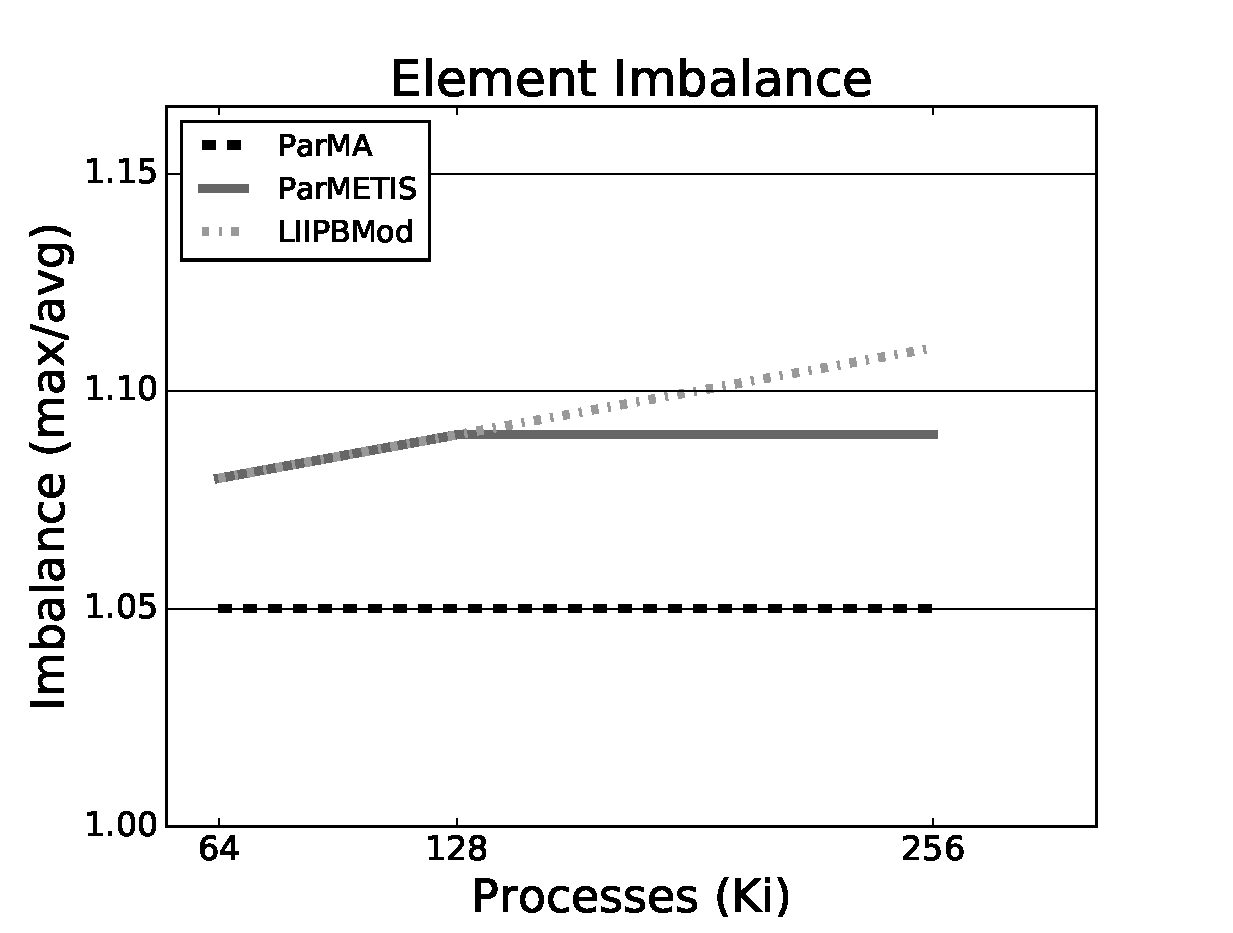
\includegraphics[width=.6\textwidth]{results/liipbmod-v-parma/elmImb.eps}
  \caption{
    Evolution of the (top) vertex and (bottom) element imbalance with ParMA,
    LIIPBMod, and ParMETIS in the 941 million element AAA mesh.
  }
  \label{fig:liipbmod-v-parma}
\end{figure}
\subsection{Feature Tests} \label{sec:featureTests}

We tested ParMA vertex$>$element improvement on a 497,058 triangular-element
MPAS North America 15km-to-75km graded ocean mesh partitioned to 1Ki parts.
The initial partition generated with local ParMETIS part k-way has a vertex and
element imbalance of 36\% and 17\%, respectively, and on average, 280 vertices
per part.

Configuration 1 of Table~\ref{tbl:oceanConfigs} serves as the baseline for
feature inclusion.
It uses iterator-based part boundary vertex traversal (disabled graph
distance), disables detection of non-manifold part junctions, has a fixed cavity
size for selection, and when balancing elements, does not cancel selections to
help preserve vertex imbalance.
Configurations 2, 3, 4, and 5 successively add the features listed in
Table~\ref{tbl:oceanConfigs}.

For each configuration Fig.~\ref{fig:oc10_16vtx} and Fig.~\ref{fig:oc10_16vtxElm}
depict the change in partition quality, relative to the initial partition,
after ParMA balancing.
ParMA's target imbalance was set to 5\% for vertices and elements.
Partition quality is measured in three ways:
(1) the average number of neighbors per part, counted via shared vertices,
`avgNB/part',
(2) the average number of vertices and edges per part, `avgVtx/part' and
`avgEdge/part', and
(3) the entity imbalance, $I^{d}$.
For each of these measures a value of one indicates no change from the initial
partition, while a value greater (lower) than one indicates an increase
(decrease) in the measure relative to the initial partition.

\begin{figure} \centering
  \begin{subfigure}[b]{.7\textwidth}
    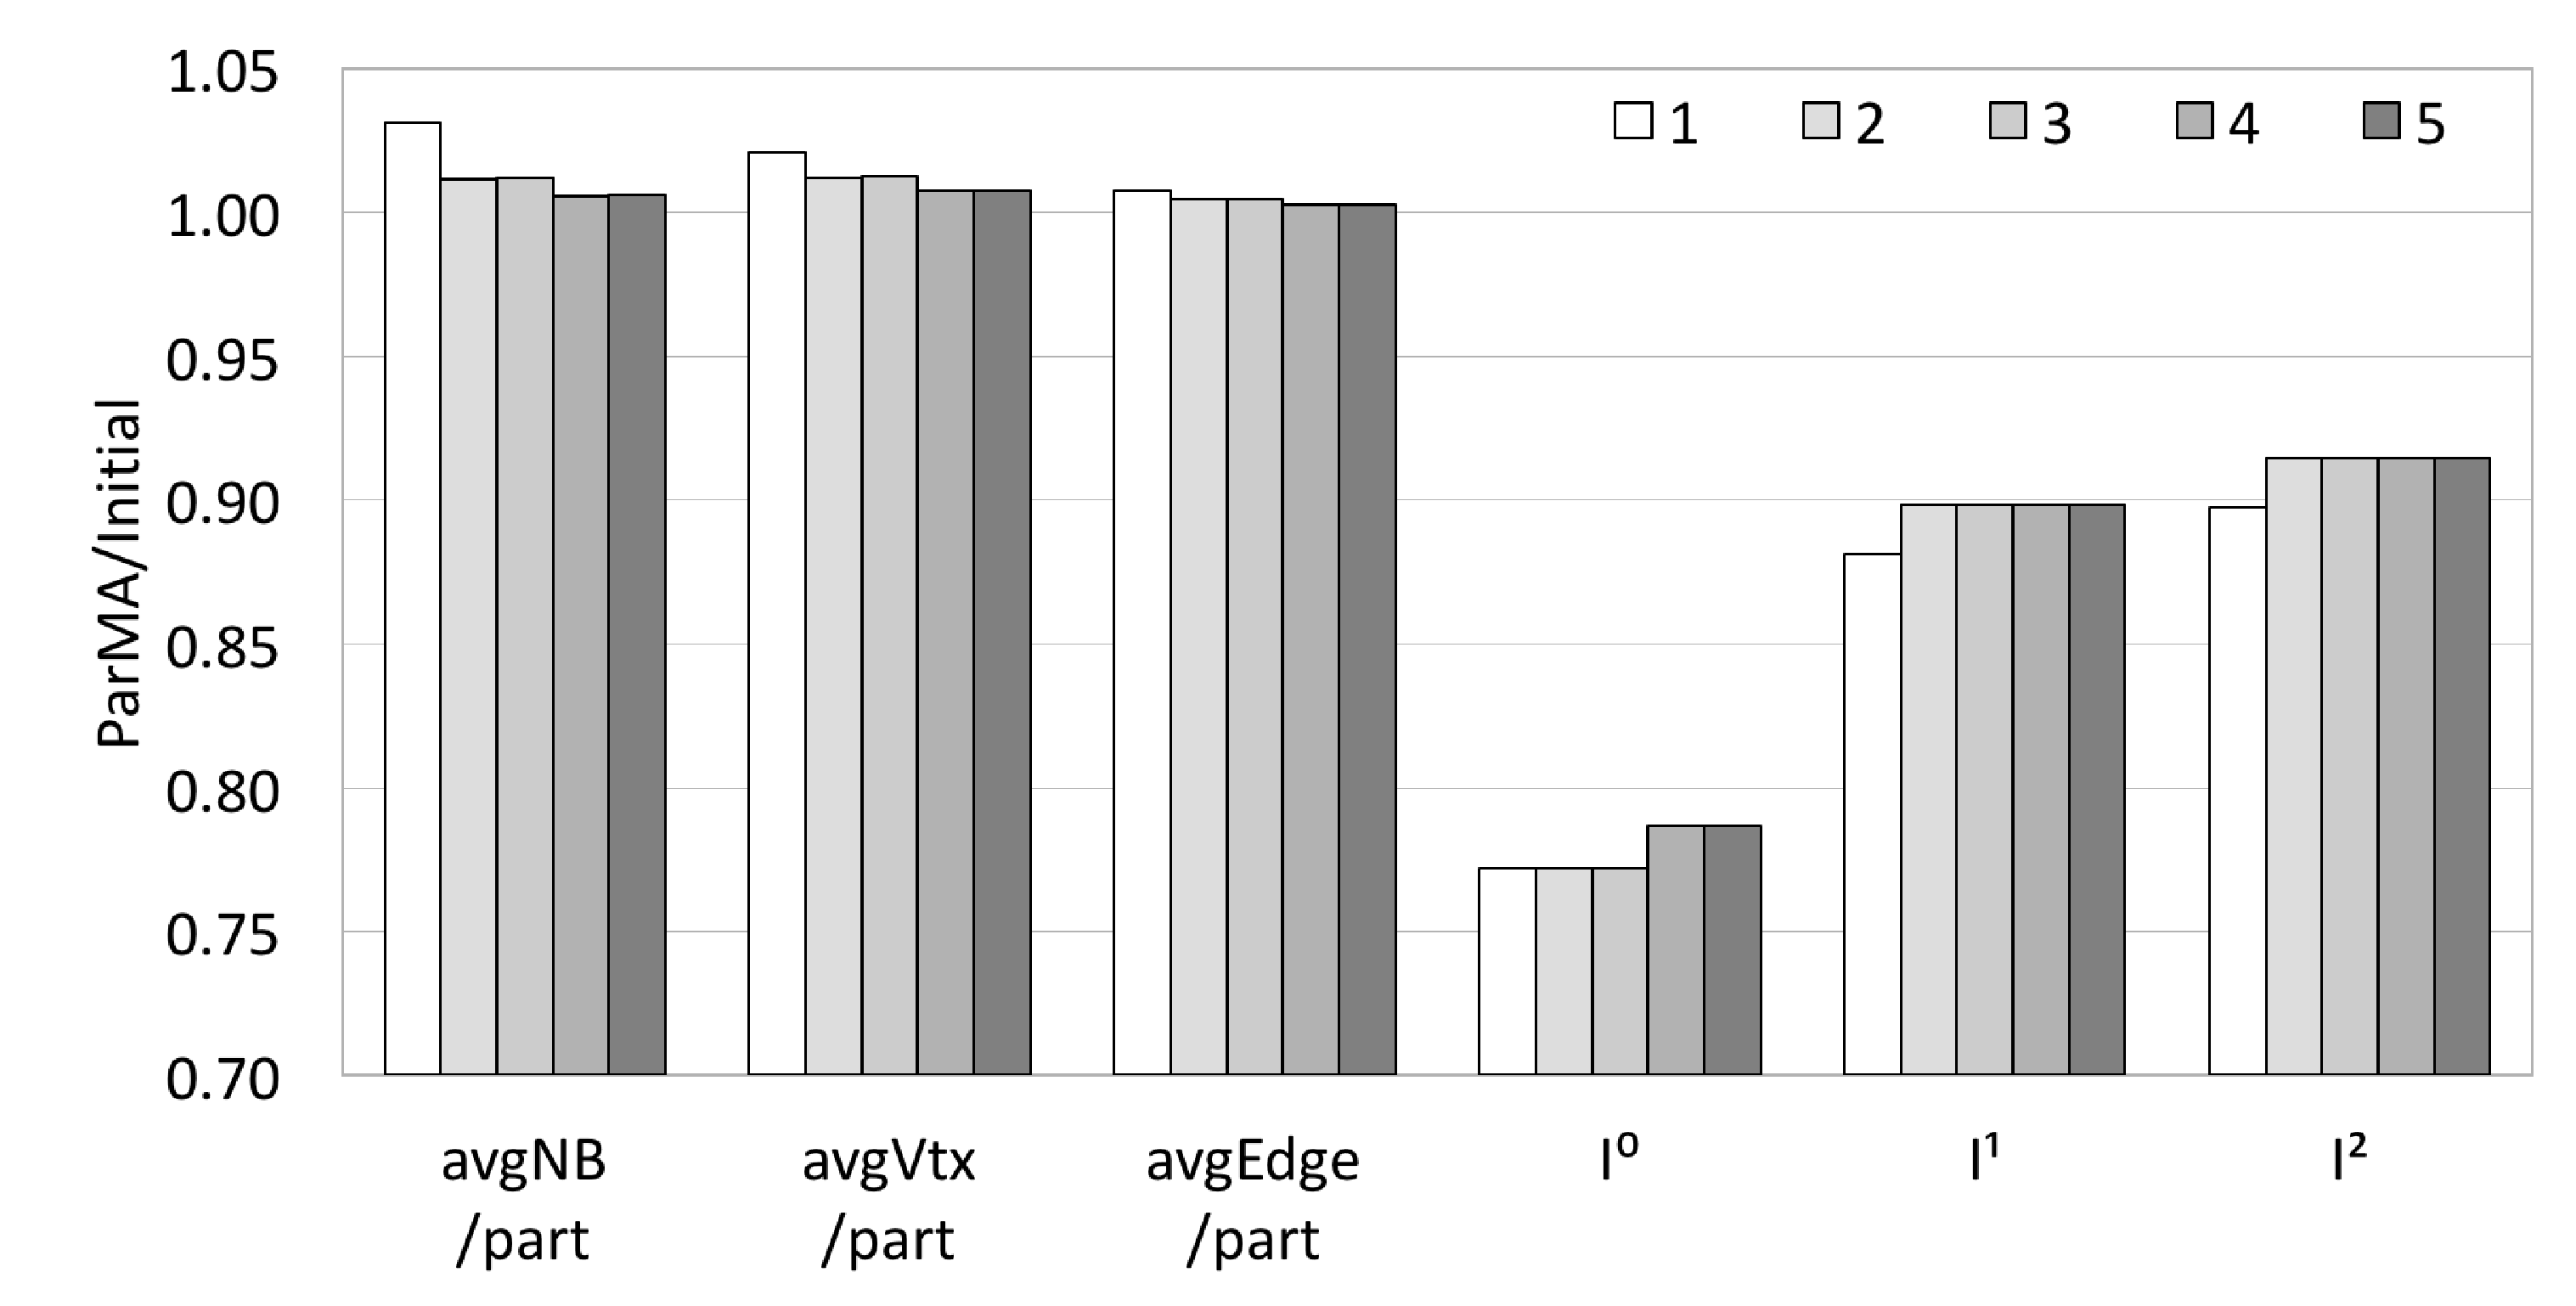
\includegraphics[width=\textwidth]{results/configTest/ocean/oc10_16_vtxVsInitial.eps}
    \caption{Partition quality after vertex balancing.}
    \label{fig:oc10_16vtx}
  \end{subfigure}
  \begin{subfigure}[b]{.7\textwidth}
    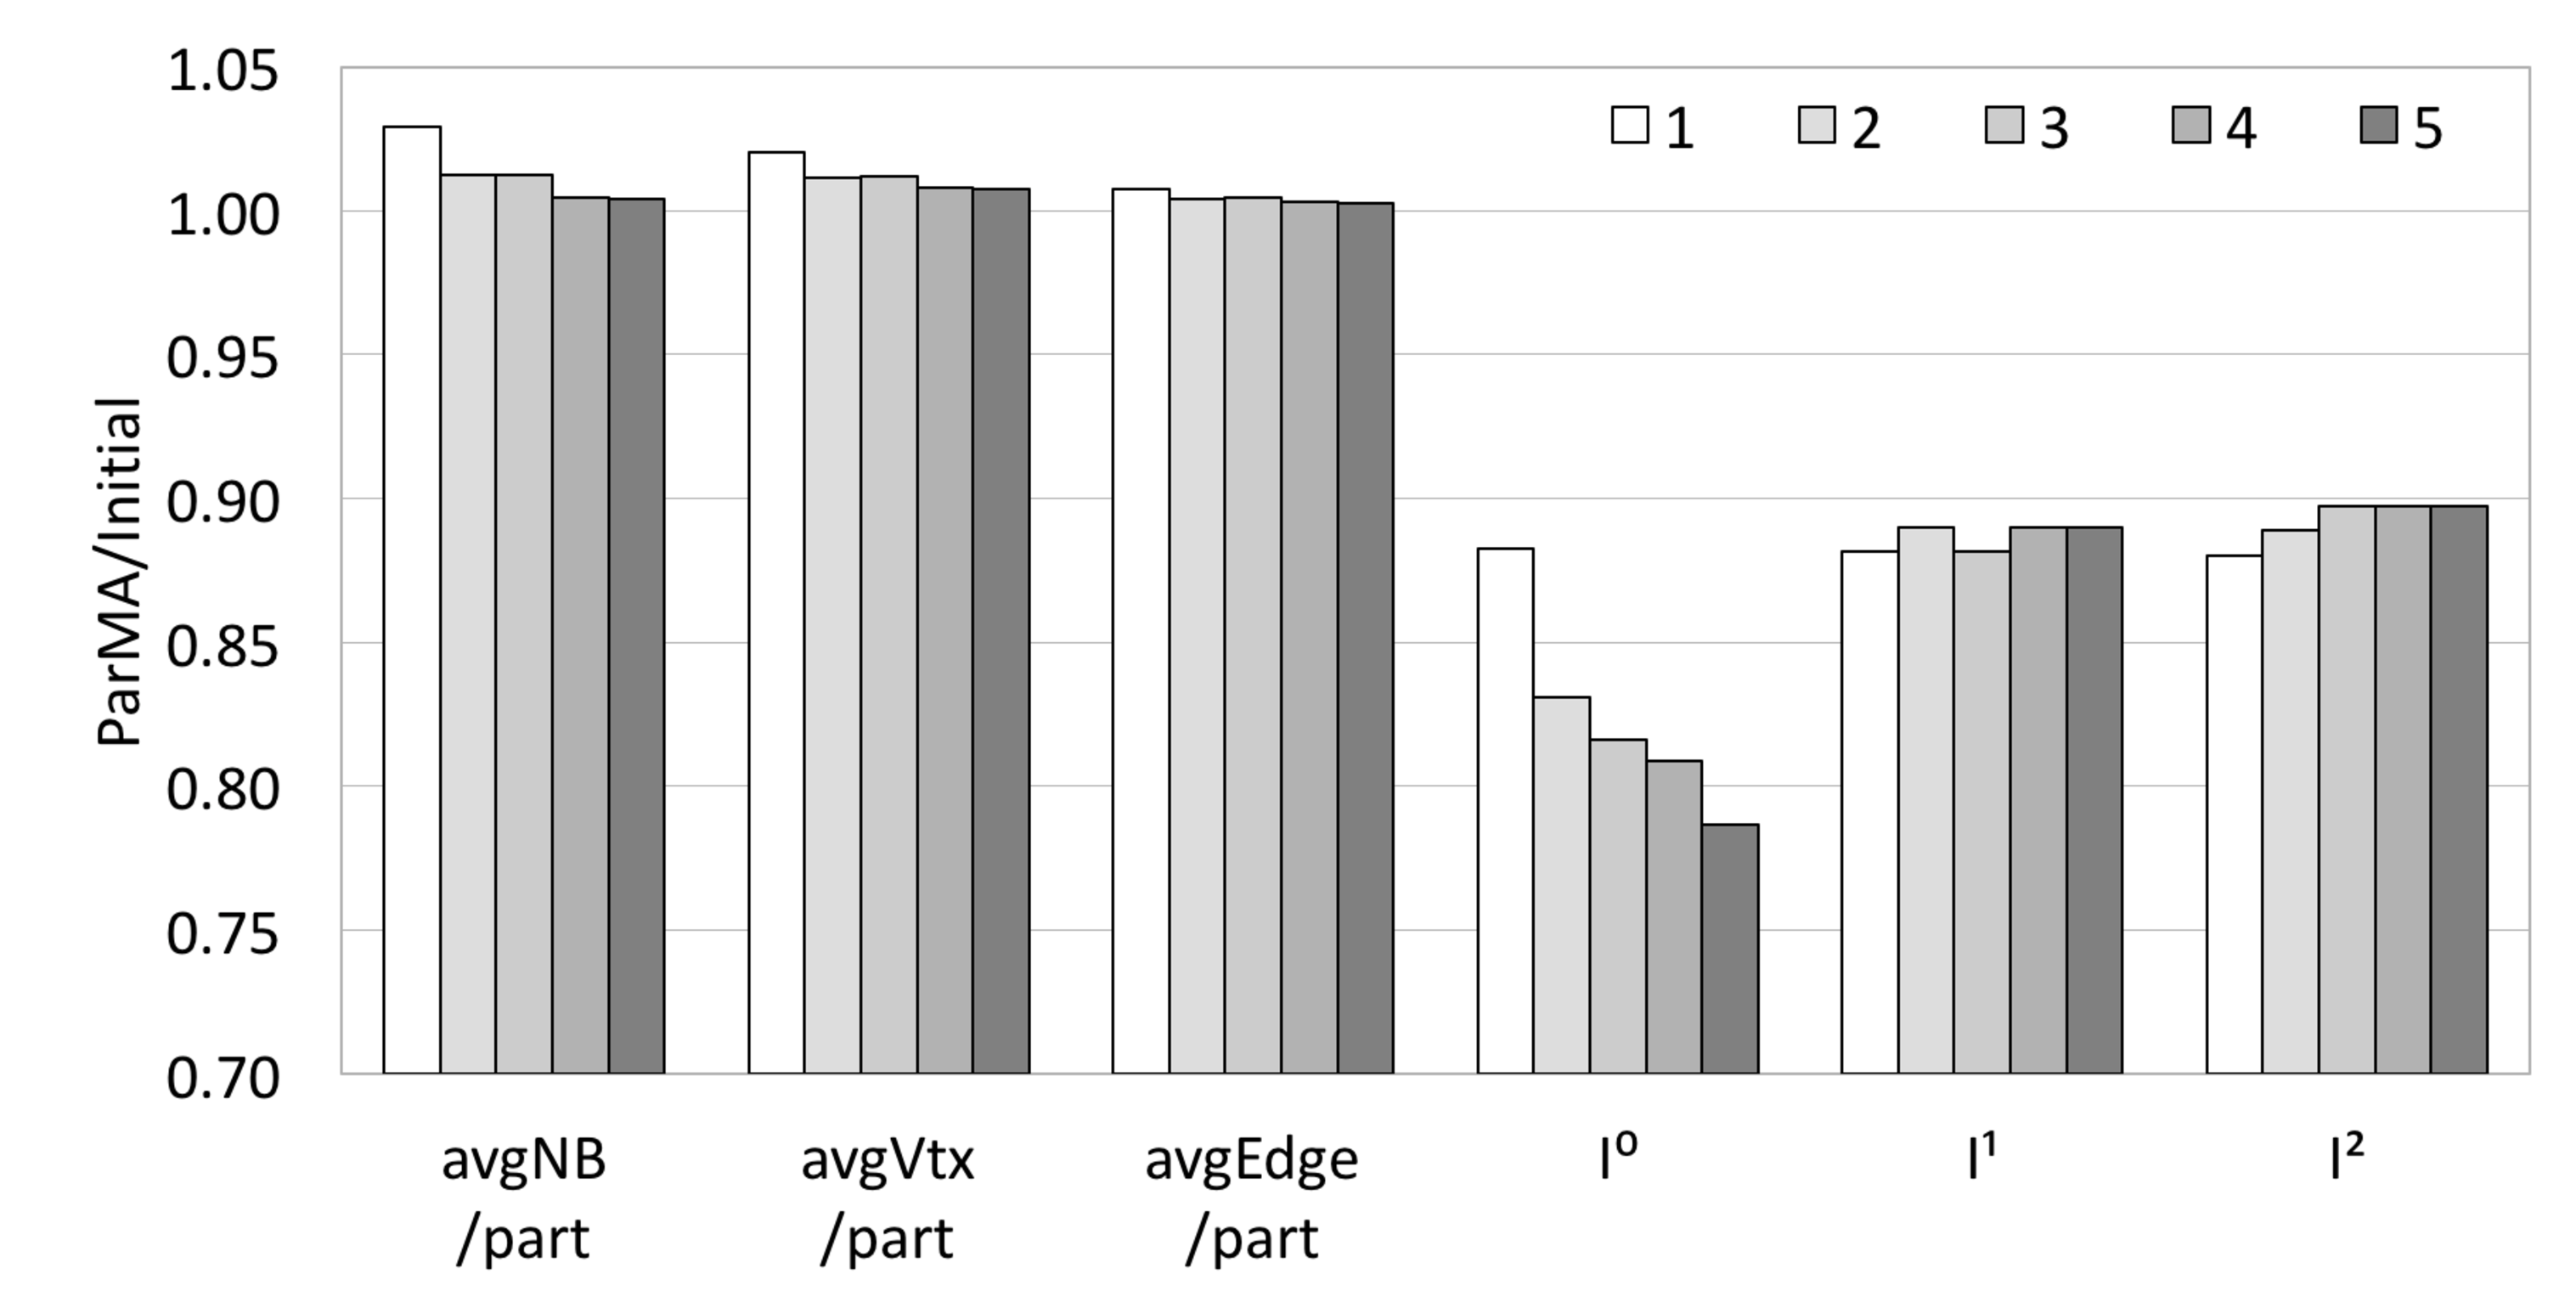
\includegraphics[width=\textwidth]{results/configTest/ocean/oc10_16_elmVsInitial.eps}
    \caption{Partition quality after vertex $>$ element balancing.}
    \label{fig:oc10_16vtxElm}
  \end{subfigure}
  \begin{subfigure}[b]{.75\textwidth}
    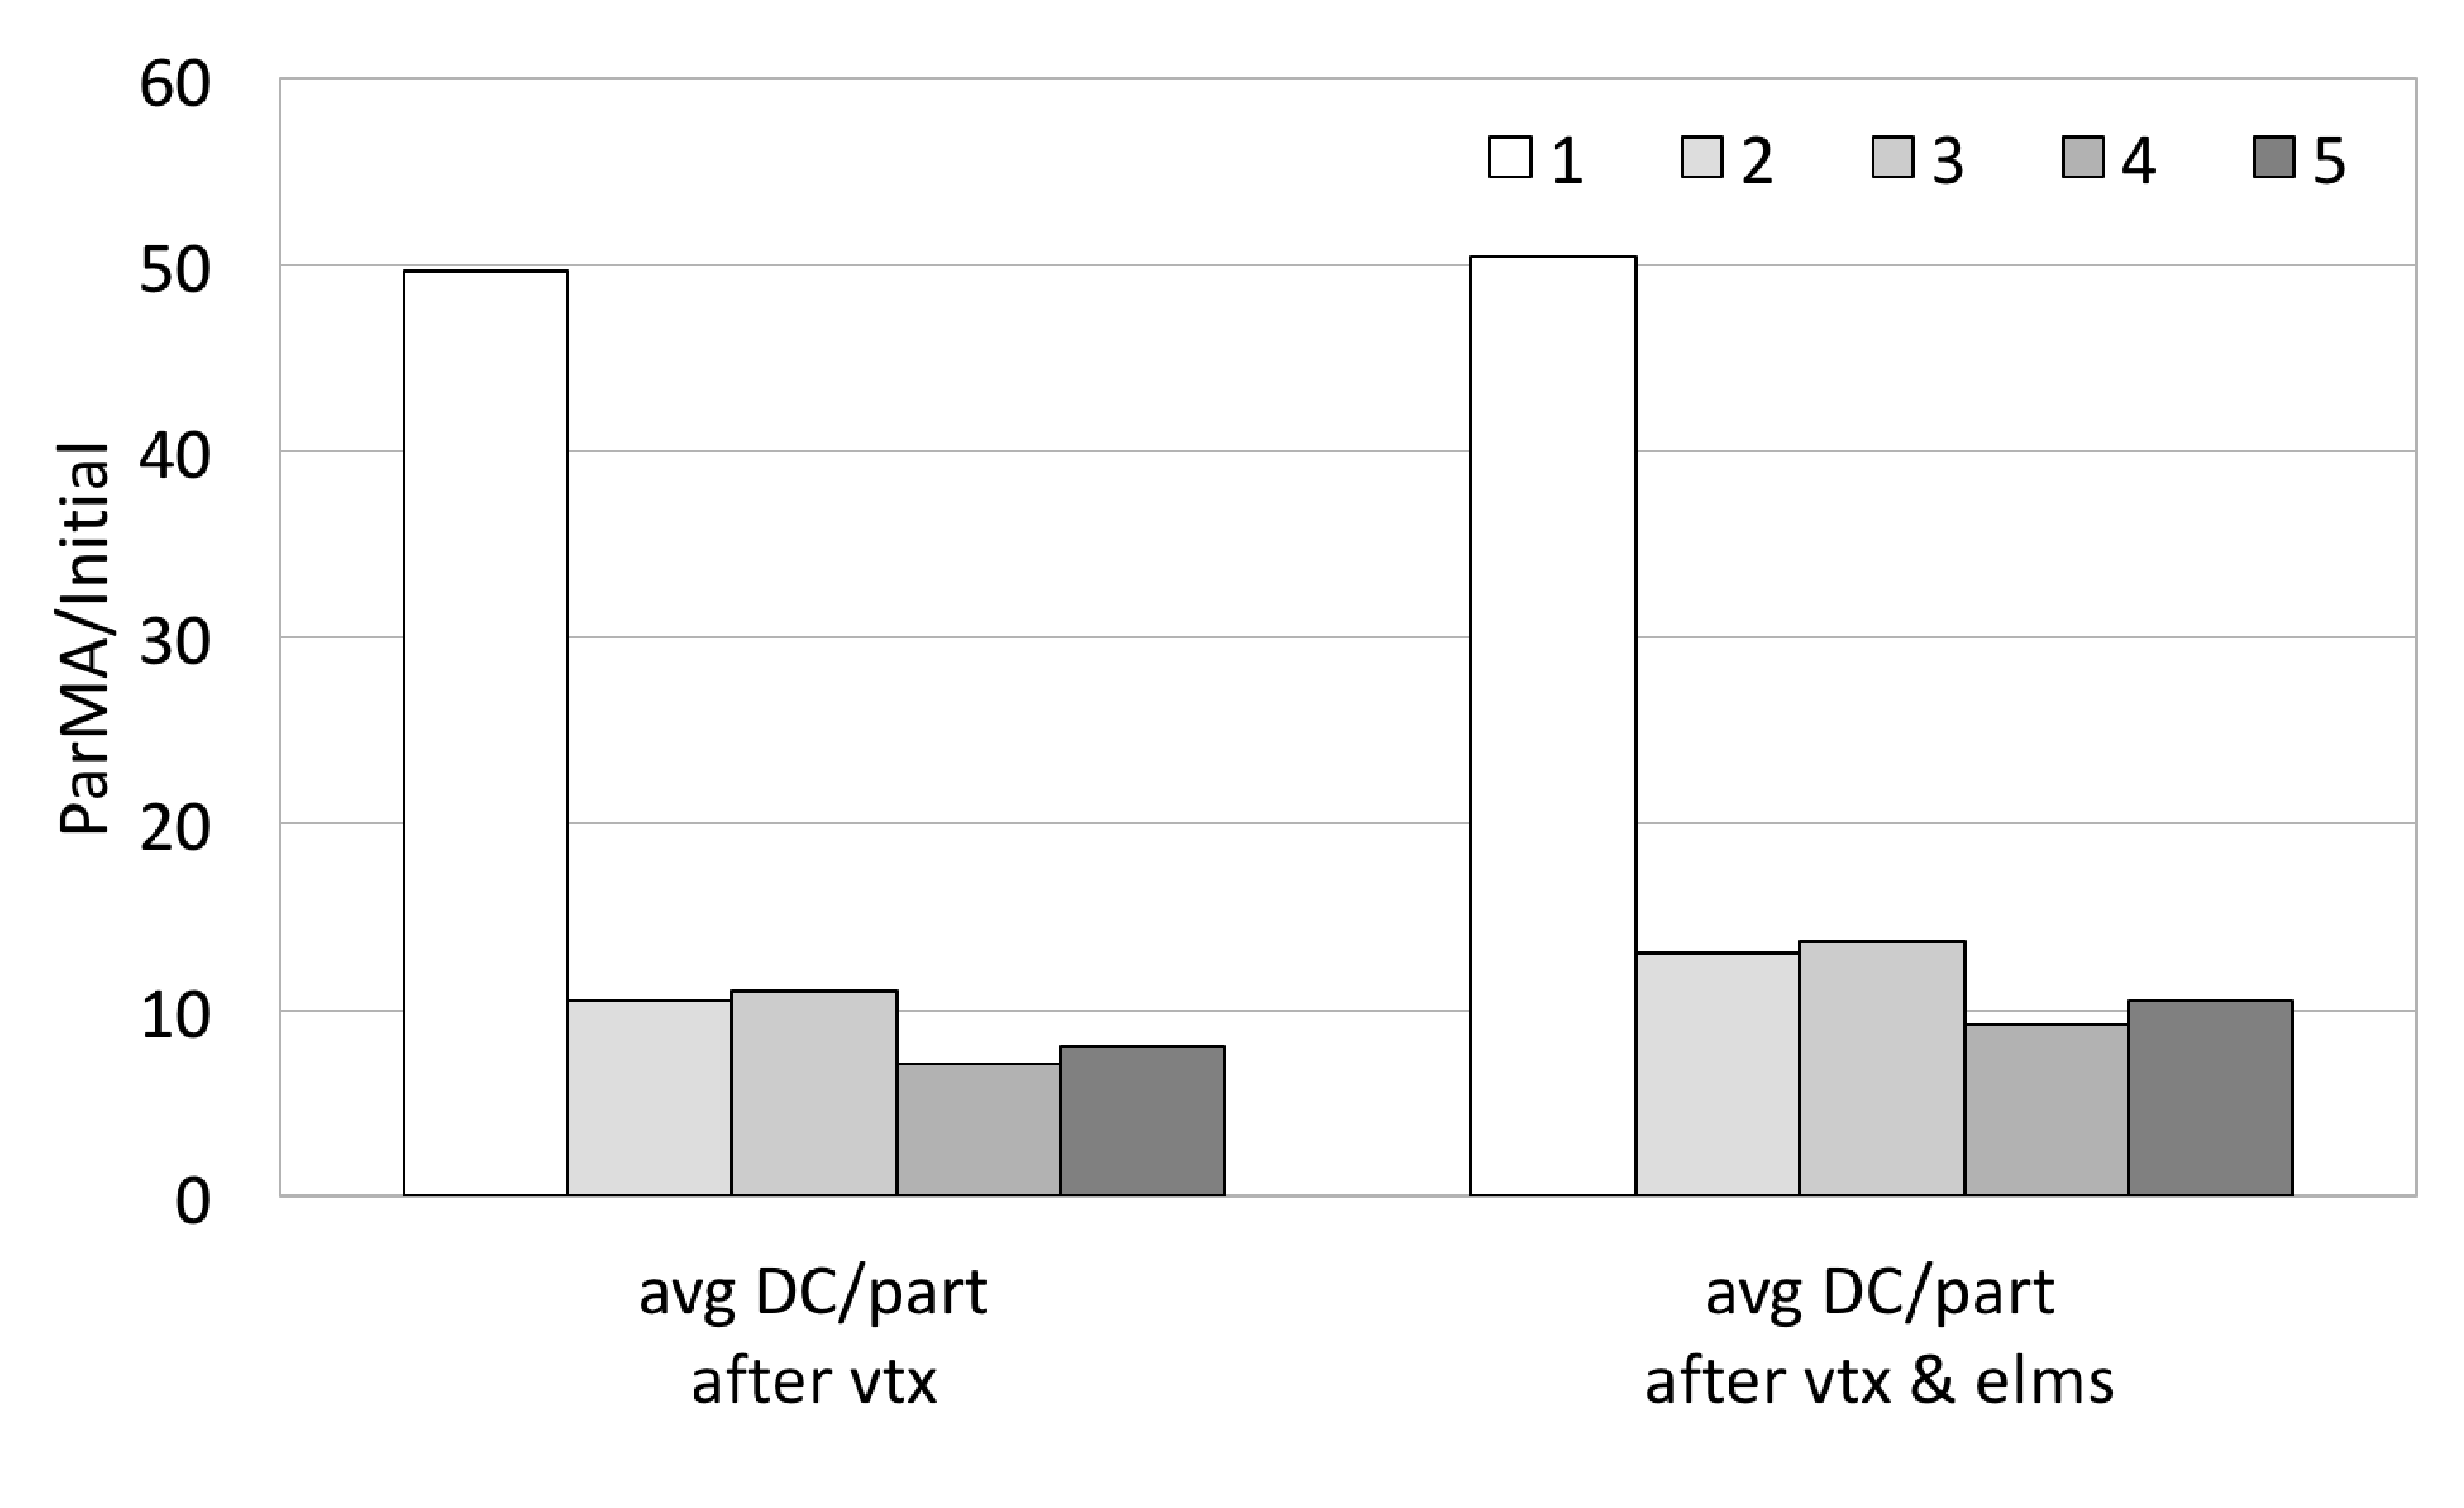
\includegraphics[width=\textwidth]{results/configTest/ocean/oc10_16_dcParts.eps}
    \caption{Disconnected components.}
    \label{fig:oc10_16dc}
  \end{subfigure}
  \caption{
    Partition quality of a 1,024 part MPAS North America 15km to 75km graded ocean mesh using
    the ParMA configurations listed in Table~\ref{tbl:oceanConfigs}.
  }
  \label{fig:oc10_16}
\end{figure}


\begin{table} \centering
  \footnotesize
  \caption{
    ParMA test configurations.
  }
  \label{tbl:oceanConfigs}
  \begin{tabular}{l | l }
    Configuration & Enabled Features \\
    \hline
    1             & None \\
    \hline
    2             & 1 + graph distance traversal\\
    \hline
    3             & 2 + non-manifold feature detection\\
    \hline
    4             & 3 + increasing cavity size selection\\
    \hline
    5             & 4 + selection cancellation \\
  \end{tabular}
\end{table}

Fig.~\ref{fig:oc10_16vtx} depicts the improvement in quality after vertex
balancing.
The average number of neighbors, vertices, and edges per part increases by one
percent or less with all features enabled.
Relative to the over 20\% decrease in vertex imbalance, these increases are
negligible.




Vertex$>$element balancing, Fig.~\ref{fig:oc10_16vtxElm}, further improves
the partition quality as features are enabled.
After Configuration 1 (element balancing with no features enabled), the element
imbalance is reduced from 5\% to 3\% at the cost of a vertex imbalance increase
from 5\% to 20\%.
Enabling graph distance traversal, Configuration 2, reduces the average
number of disconnected components per part.
Fig.~\ref{fig:oc10_16dc} shows that the disconnected component count,
relative to the initial partition, increases by 50x in Configuration 1 while
Configuration 2 only has a 10x increase.
The large reduction in disconnected components reduces the number of vertices on
the part boundaries.
This reduction in turn helps limit the vertex balance increase to 13\% after
element balancing.
The features of Configuration 4 further reduce the number
of boundary vertices (as indicated by the reductions in average neighbors,
edges, and vertices per part) and results in a 10\% vertex imbalance.
With all features enabled, Configuration 5, a final vertex imbalance of 7\% is
reached while maintaining the 5\% element imbalance and further improving
the other quality measures.
This Configuration runs in 72\% of the time of Configuration 1; 3.07 seconds versus
4.25 seconds.
The faster run time is mainly the result of vertex balancing times reducing from
4.09 seconds to 2.82 seconds, and only a slight increase in the element
balancing times from 0.16 seconds to 0.25 seconds.

We also ran the feature test on the 3D 2.3 million element RPI Formula Hybrid
suspension upright mesh, the geometric model depicted in
Fig.~\ref{fig:upright}. 
The test mesh has 2,048 parts and a 46\% vertex and 10\% element initial
imbalance.
ParMA's target imbalance was set to 5\% for both vertex and vertex$>$element
balancing.
Fig.~\ref{fig:up11_32} shows the results of the tests.
In Configuration 1 balancing the mesh vertices to 10\% increases the element
imbalance to 26\%.
The subsequent element balancing reduces the element imbalance to 5\% in 17.8
seconds, but increases the vertex imbalance to 29\%.
As features are enabled the partition quality and imbalances improve at the cost
of increased run time.
Running with all features enabled (Configuration 5) requires 37.6 seconds (two
times longer than Configuration 1), and reaches an element imbalance of 5\% and
a vertex imbalance of 9\%.

\begin{figure} \centering
  \begin{subfigure}[b]{.7\textwidth}
    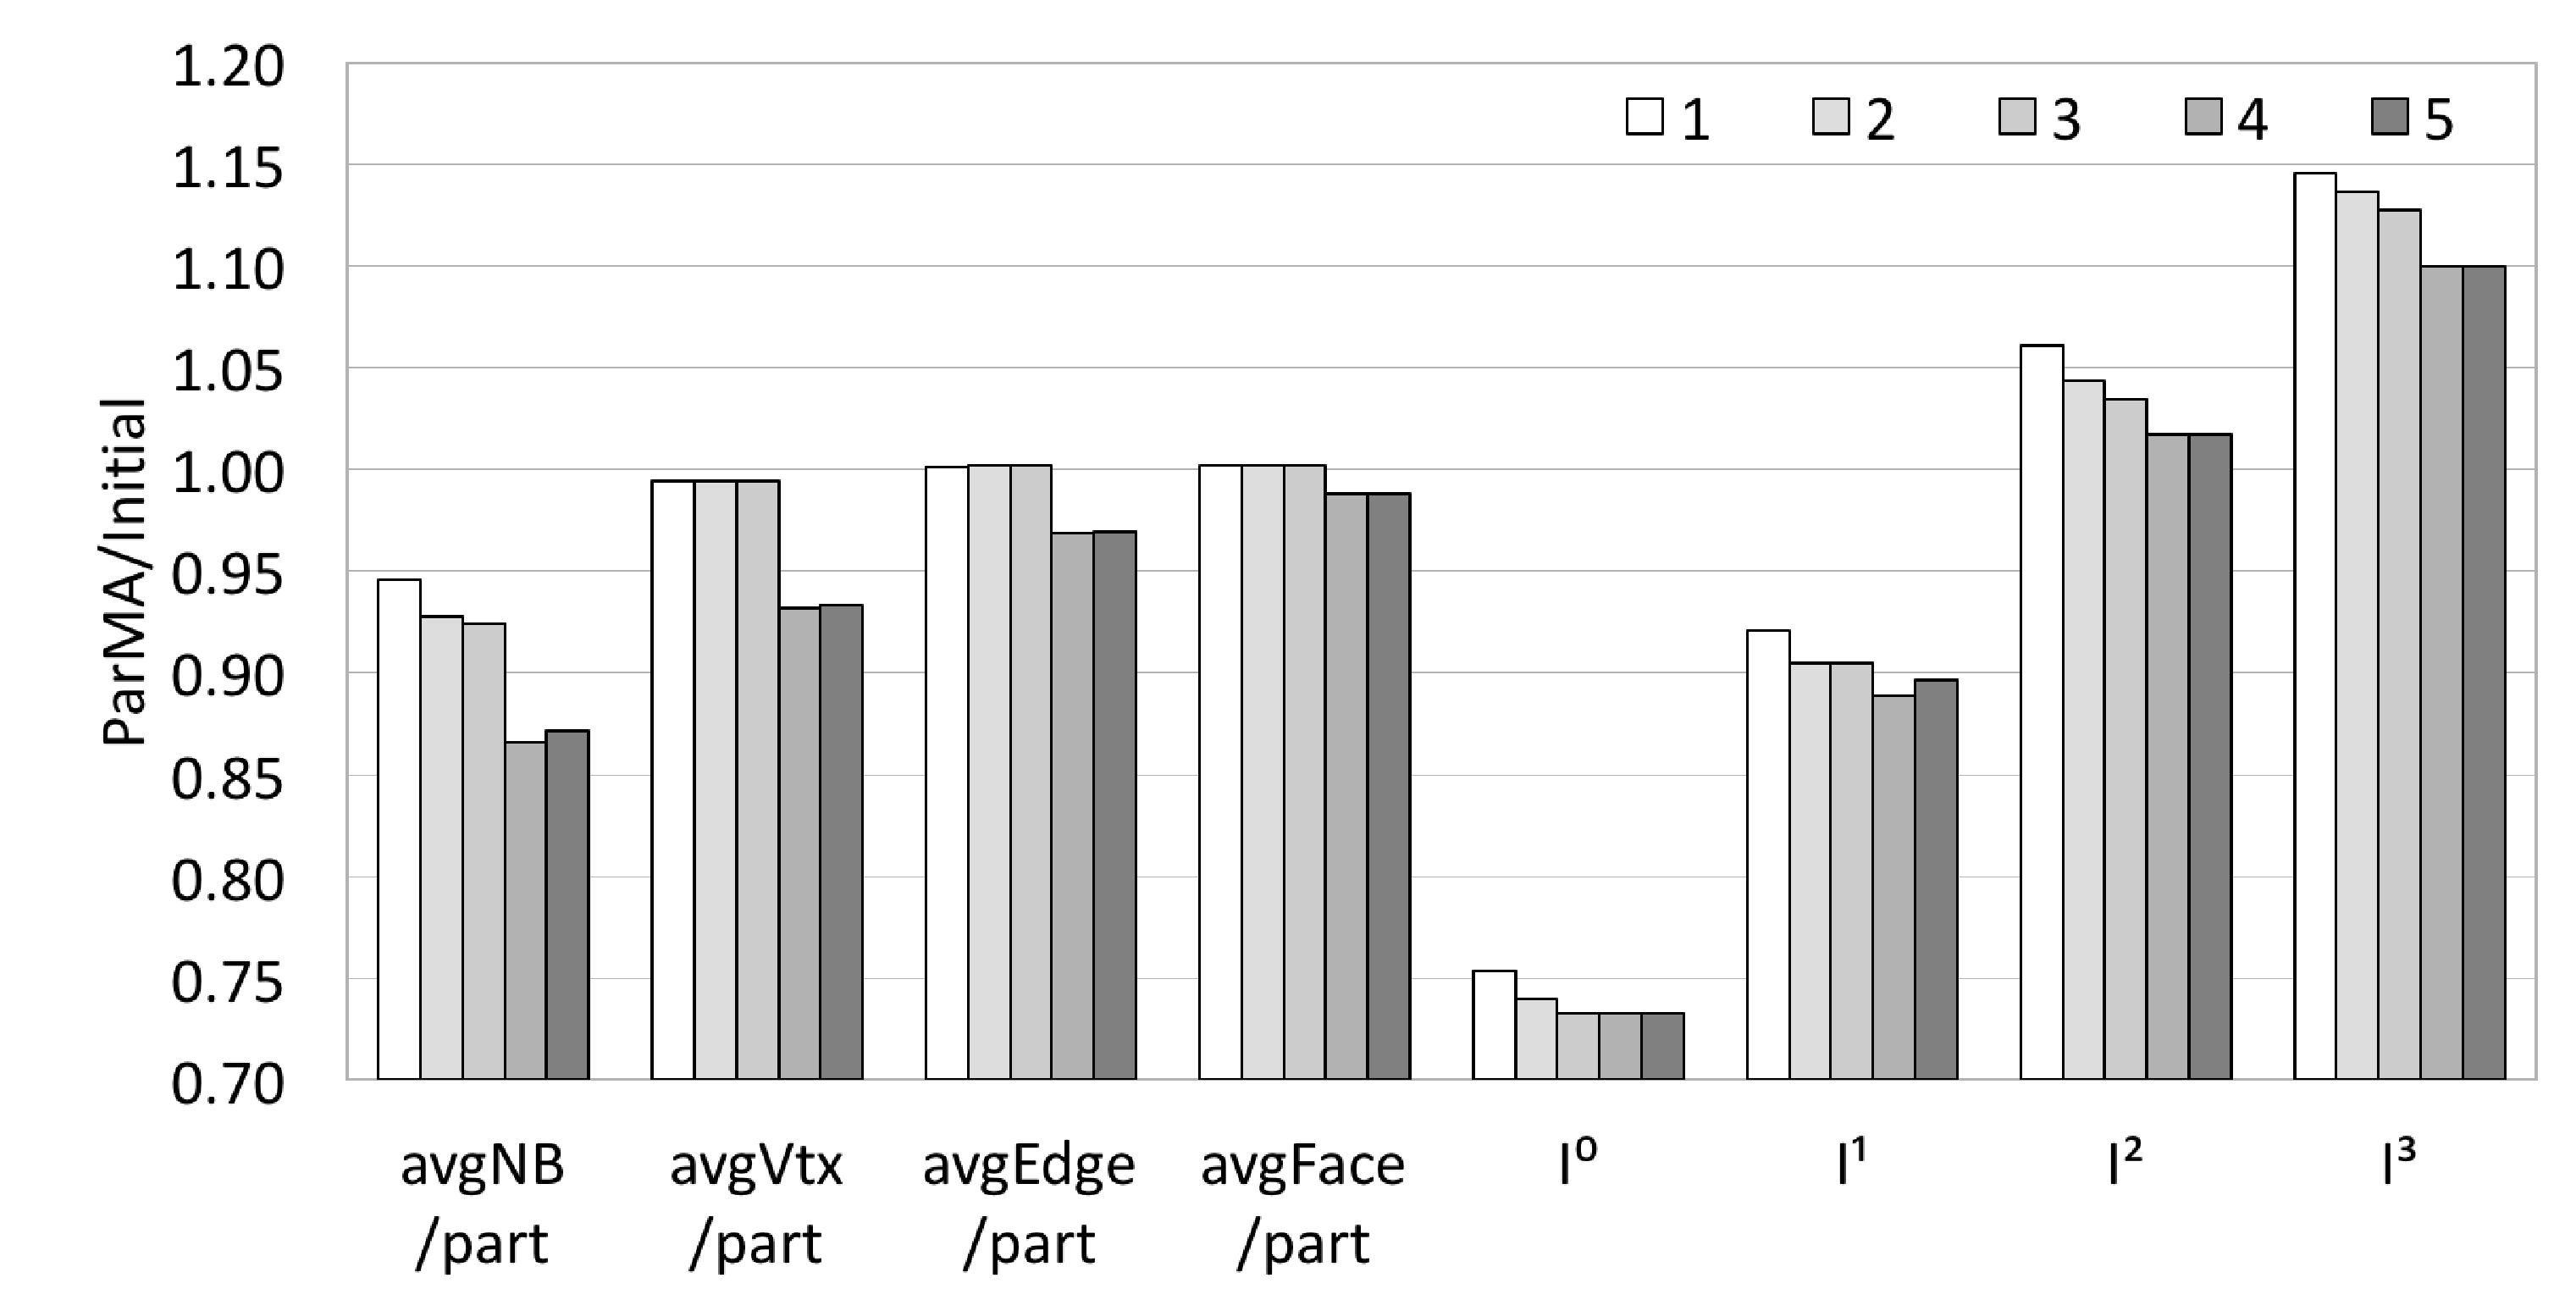
\includegraphics[width=\textwidth]{results/configTest/up11/up11_32_vtxVsInitial.eps}
    \caption{Partition quality after vertex balancing.}
    \label{fig:up11_32vtx}
  \end{subfigure}
  \begin{subfigure}[b]{.7\textwidth}
    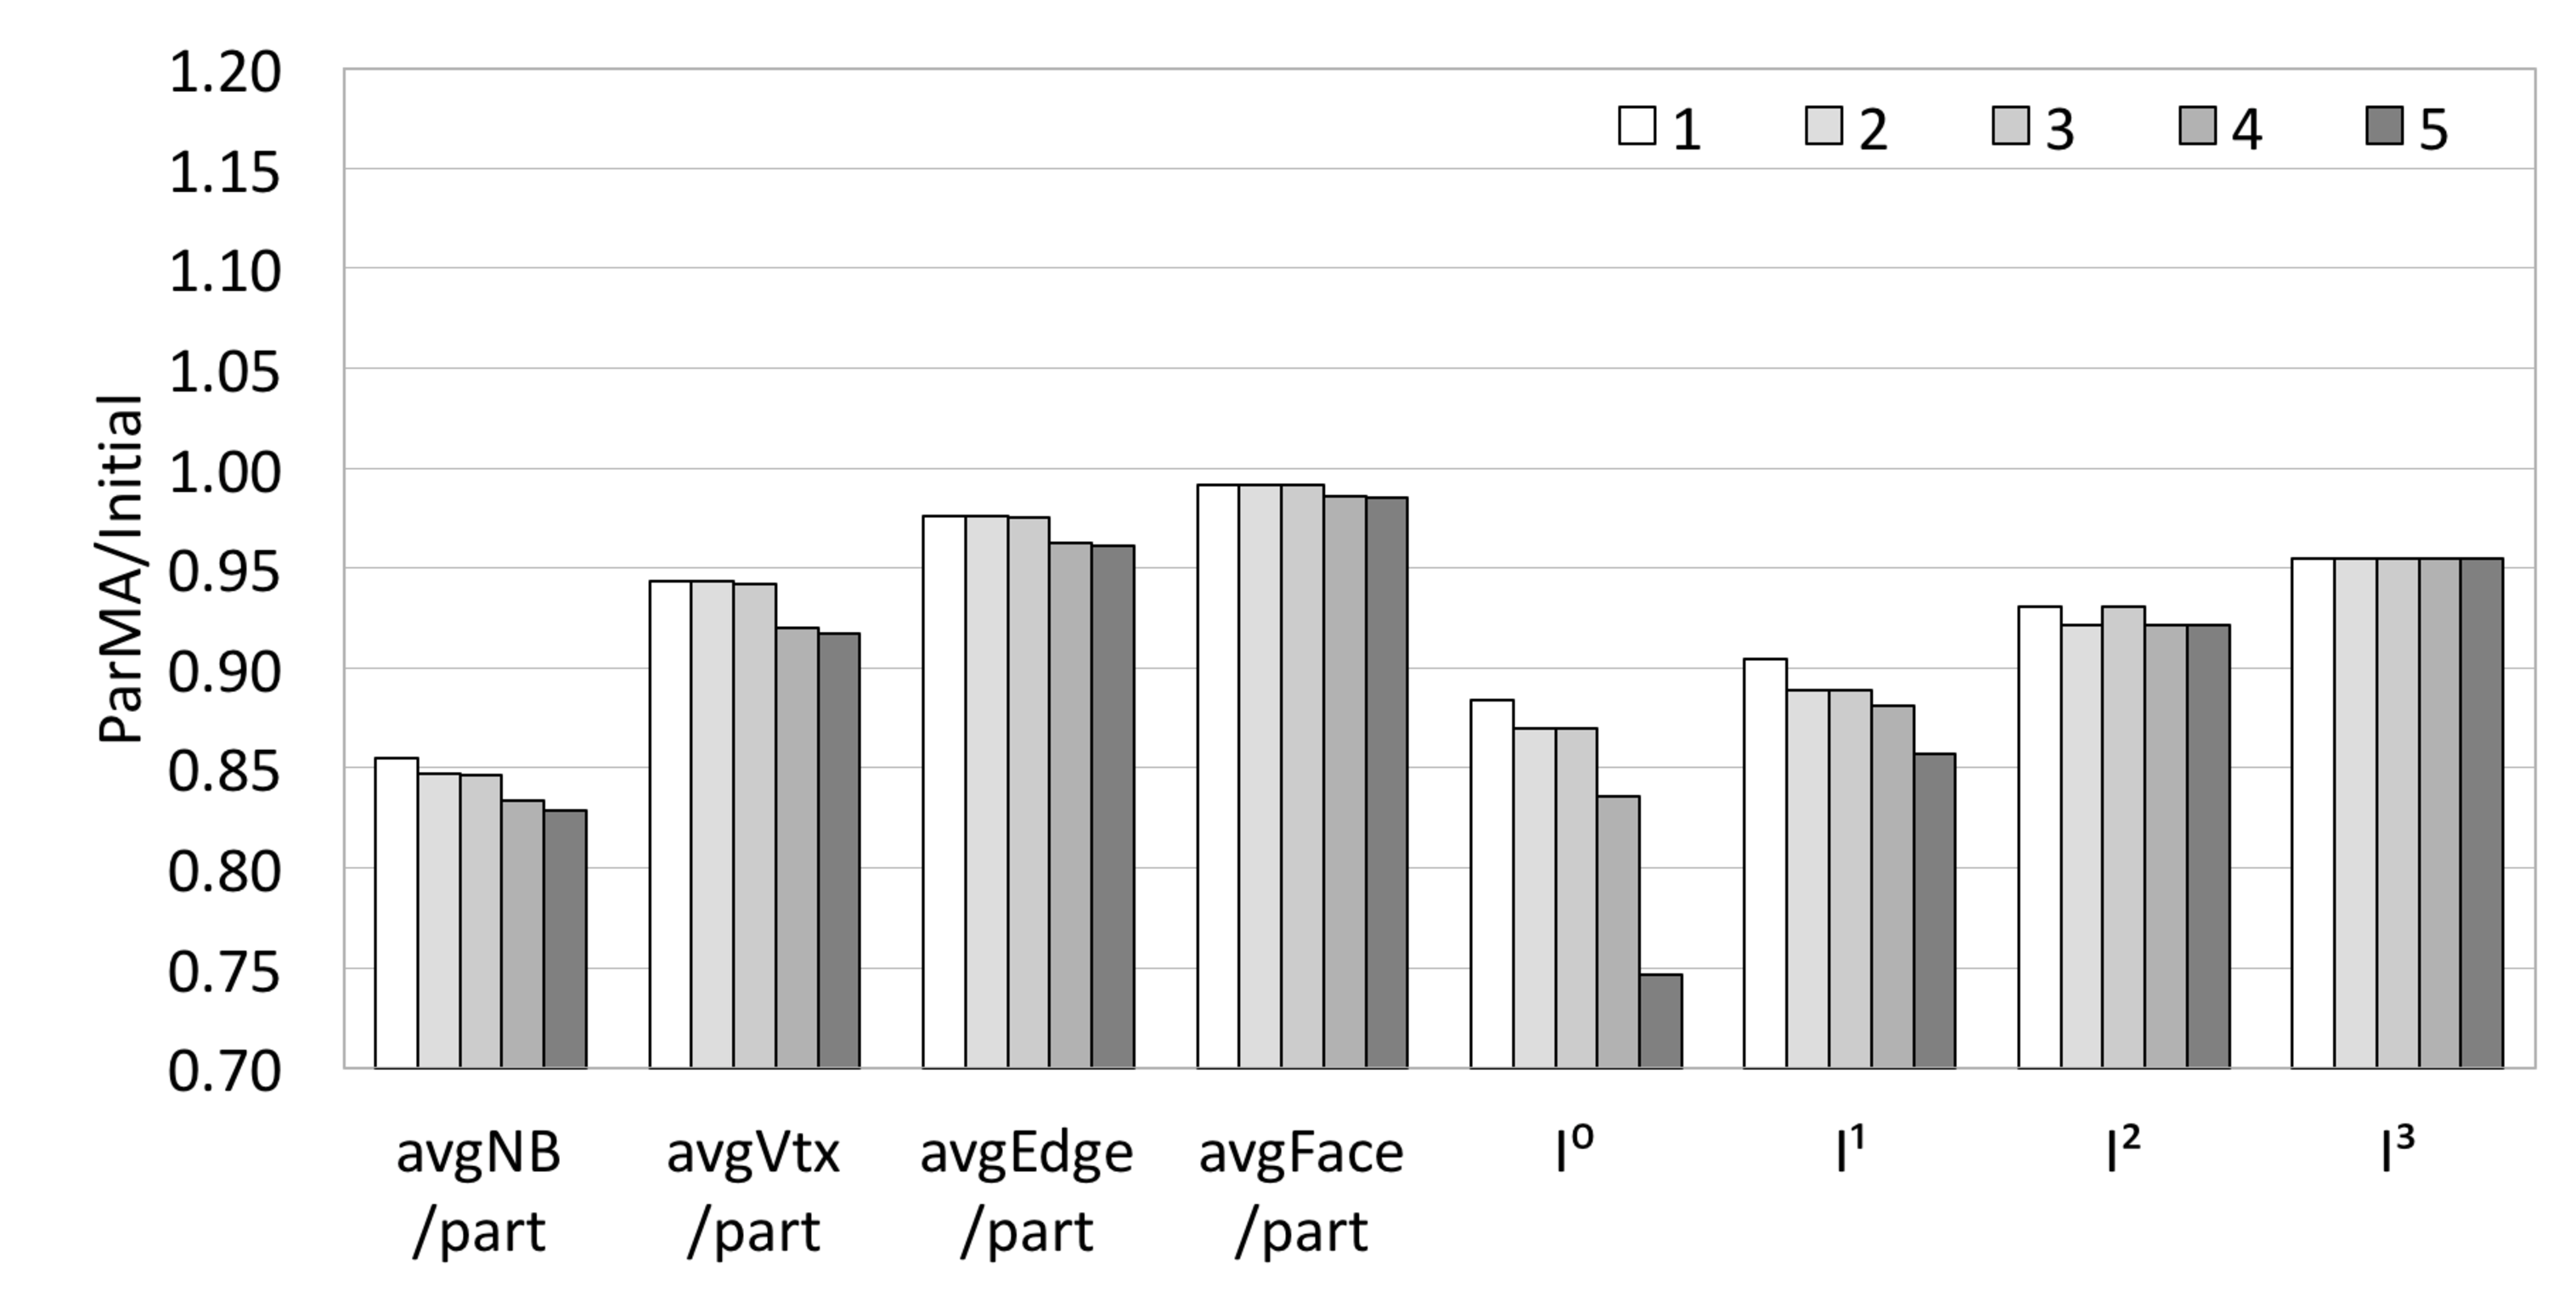
\includegraphics[width=\textwidth]{results/configTest/up11/up11_32_elmVsInitial.eps}
    \caption{Partition quality after vertex $>$ element balancing.}
    \label{fig:up11_32vtxElm}
  \end{subfigure}
  \begin{subfigure}[b]{.75\textwidth}
    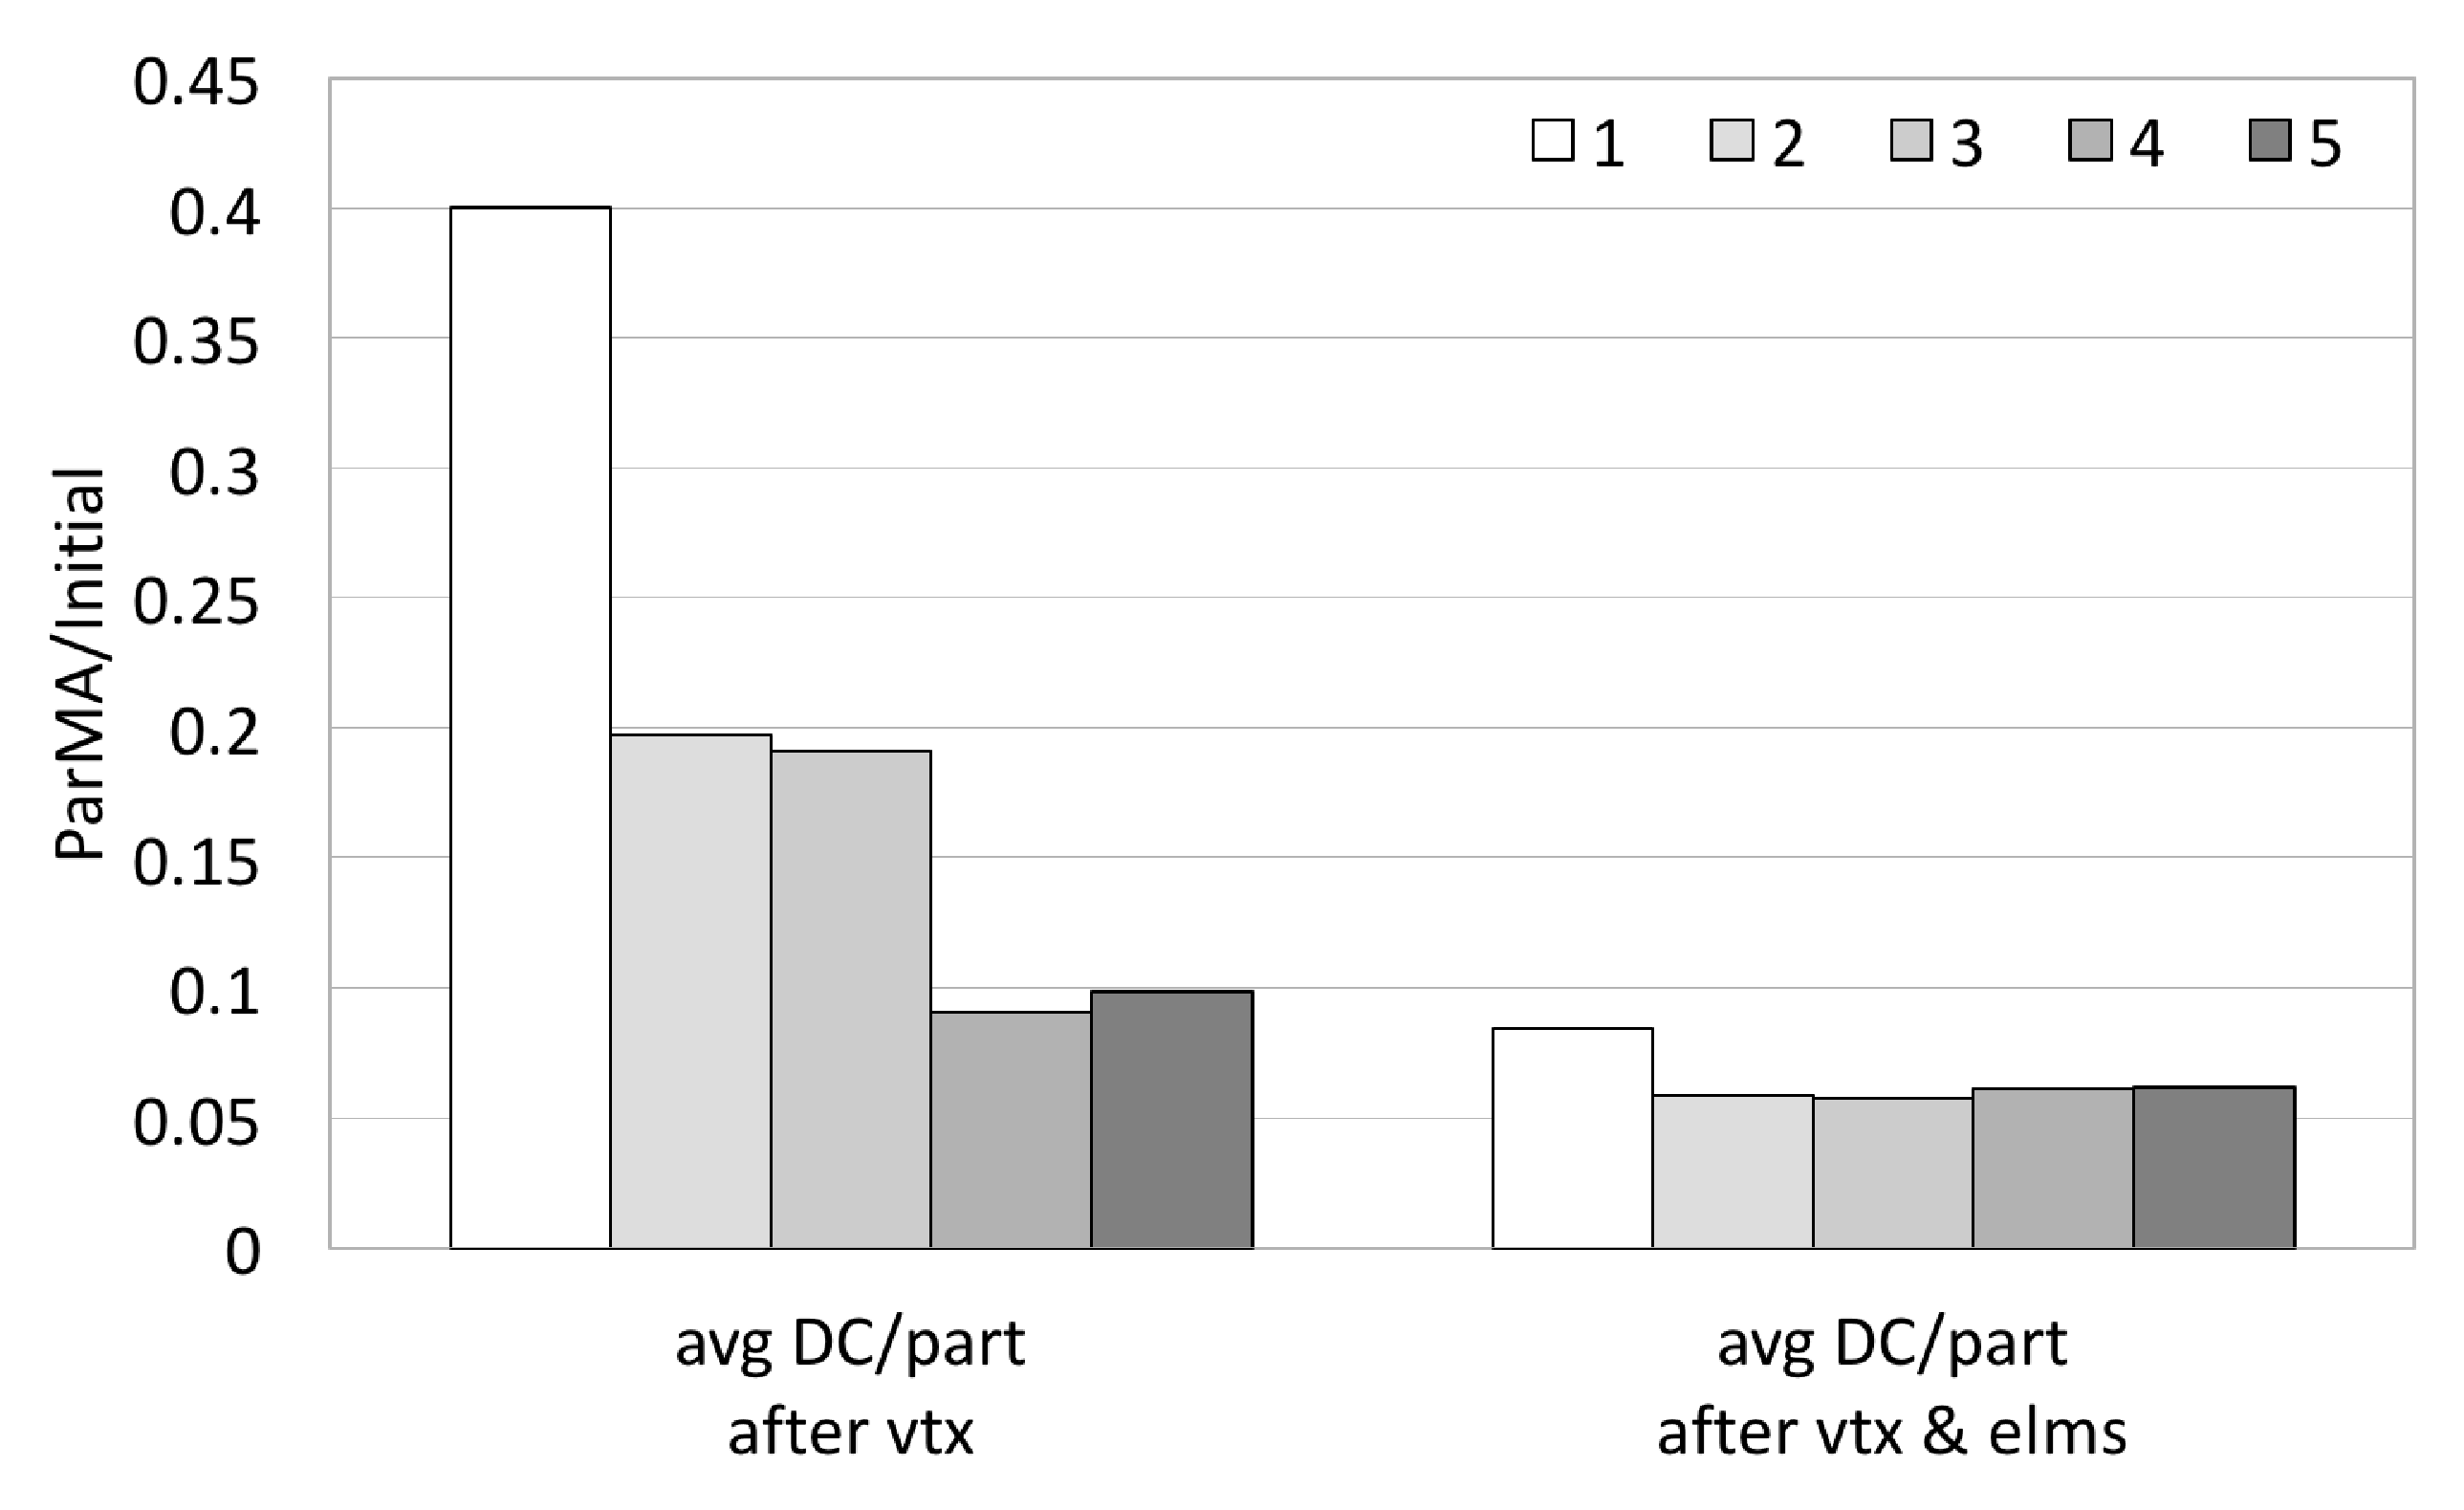
\includegraphics[width=\textwidth]{results/configTest/up11/up11_32_dcParts.eps}
    \caption{Disconnected components.}
    \label{fig:up11_32dc}
  \end{subfigure}
  \caption{
    Partition quality of a 2,048 part RPI Formula Hybrid suspension upright mesh
    using the ParMA configurations listed in Table~\ref{tbl:oceanConfigs}.
    Lower is better.
  }
  \label{fig:up11_32}
\end{figure}

A critical difference of the 3D upright tests to the 2D MPAS tests is the large
reduction in disconnected parts and the related decrease in the average
neighbors and entities per part.
Compared to the initial partition, Configuration 5 of the upright test reduces
the average neighbors, vertices, and disconnected components per part by 17\%,
8\%, and 93\% respectively, and 3\%, 2\%, and 27\% versus Configuration 1.
This difference is mostly due to the change from 2D to 3D and the increased
connectedness of the geometric model that enables more migration opportunities;
the MPAS mesh has multiple geometric surfaces which only share one or two
vertices with other surfaces.

The feature tests were run using one part per core on the Blue Gene/Q at the
Rensselaer Center for Computational Innovations.
Tests with all features enabled and additional balancing criteria are described next.

\subsection{Multi-Criteria Improvement}

Analysis codes which have work associated with multiple entity dimensions and have a
non-uniform distribution of that work require multi-criteria balancing.
Codes with this requirement include finite elements with
non-uniform \textit{p}, particle-in-cell~\cite{worleyBalancePic2016},
contact/impact~\cite{fingbergContact2000},
atomistic-to-continuum~\cite{FrantzDale2010}, and other multi-model or
multi-physics techniques~\cite{chevalier2012load}.
ParMA satisfies this requirement by balancing the entity dimensions defined in
a priority-sorted list.
For each entity in the mesh the application also optionally provides weights
specifying the associated computational load.
To test this ability we ran ParMA vertex$=$edge$>$element balancing on a 2.3 million
element, 2,048 part mesh of the suspension upright.
The test emulates a non-uniform work distribution associated with edges by
setting entity weights.
On part zero edge weight is set to two; all other parts have entity weights of
one.

Two initial partitions were used in testing; one is the result of mesh adaptation
(listed as `adapt'), and another is generated with RIB.
The partitions' average entity counts and imbalances are listed in
Table~\ref{tbl:veeb}.
The adapt partition, relative to the RIB partition, has a ten point higher
element imbalance, and on average, four more neighbors and two more disconnected
components per part.
Given the lower initial quality, ParMA improvement on the adapt partition
requires about 350\% more time to run (27.4 seconds versus 7.7 seconds), and has 
final entity imbalances (noted in the `elements' row) a few points
higher than the final ParMA imbalances of the RIB partition.
Note, even with the run time increase, the time spent in ParMA is insignificant
relative to the time spent executing a typical finite element analysis
on a partition of this size.

Despite an initial weighted-edge imbalance of over 90\% in both partitions, ParMA
reduces the entity imbalances to less than 9\% while also reducing the average
per part entity weights by up to 5\%.
Critical to this result is ParMA's ability to diffuse away edge weight from the
heavily imbalanced part zero while not overloading other parts. 
Diffusion reduces the number of mesh edges in part zero from 1674 to 901 in
the adapt partition, and from 1665 to 889 in the RIB partition.

\begin{table} \centering
  \footnotesize
  \caption{
    vertex$=$edge$>$element partition improvement on a 2.3 million element, 2048 part, mesh
    of the RPI Formula Hybrid suspension upright of Fig.~\ref{fig:upright}.
  }
  \label{tbl:veeb}
  \begin{tabular}
    { | l    | F{3}{1} | F{4}{1} | F{4}{1} | l | l | l | l | F{2}{2} | }
    \hline
             & \multicolumn{3}{c|}{avg/part} &       &       &       &       & \\
               \cline{2-4}
    stage    & {vtx}              & {edge}              & {face}              & I$^0$           & I$^1$           & I$^2$           & I$^3$           & {time (s)} \\ \hline
    \hline
    adapt    & {\textbf{357.749}} & {\textbf{1741.012}} & {\textbf{2497.981}} & {\textbf{1.46}} & {\textbf{1.92}} & {\textbf{1.15}} & {\textbf{1.10}} & \\ \hline
    vertices & 334.017            & 1687.742            & 2469.308            & 1.08            & 1.92            & 1.16            & 1.19            & 10.268933\\ \hline
    edges    & 330.493            & 1679.033            & 2464.258            & 1.09            & 1.06            & 1.09            & 1.13            & 6.884525\\ \hline
    elements & {\textbf{328.829}} & {\textbf{1674.661}} & {\textbf{2461.637}} & {\textbf{1.09}}   & {\textbf{1.06}}  & {\textbf{1.07}} & \textbf{1.08}   & 10.256166\\ \hline
    \hline
    RIB      & {\textbf{350.457}} & {\textbf{1737.694}} & {\textbf{2503.369}} & {\textbf{1.53}} & {\textbf{1.92}} & {\textbf{1.10}} & {\textbf{1.00}} & \\ \hline
    vertices & 337.800            & 1705.029            & 2483.359            & 1.04            & 1.95            & 1.07            & 1.10            & 3.008885\\ \hline
    edges    & 333.189            & 1692.807            & 2475.781            & 1.06            & 1.05            & 1.04            & 1.07            & 3.864137\\ \hline
    elements & {\textbf{331.387}} & {\textbf{1687.526}} & {\textbf{2472.306}} & {\textbf{1.07}} & {\textbf{1.05}} & {\textbf{1.04}} & {\textbf{1.04}} & 0.848957 \\ \hline
  \end{tabular}
\end{table}

\subsection{Partitioning to Over One Million Parts}

ParMA quickly reduces large imbalances and improves part shape of a 1.6 billion
element suspension upright mesh partitioned from 128Ki to 1Mi
(2$^{20}$) parts (approximately 1500 elements/part).
The initial 128Ki partition has less than 7\% imbalance for all entity
dimensions.
We ran the tests on the Mira Blue Gene/Q located at the ALCF.
One hardware thread was used per part.
\begin{itemize}
  \item Partitioning with global RIB completes in 103 seconds and results in a
    209\% vertex imbalance and a perfect element imbalance.
    ParMA runs on 1Mi processors in 20 seconds and reduces the vertex imbalance
    to 6\%, only increases the element imbalance to 4\%, and reduces the average
    number of vertices per part by 5.5\%.
  \item Local partitioning with ParMetis (one serial instance of ParMETIS for each
    initial part) completes in 9.0 seconds and results in a 63\% vertex
    imbalance and a 12\% element imbalance.
    ParMA runs in parallel on 1Mi processors in 9.4 seconds and reduces the
    vertex imbalance to 5\%, the element imbalance to 4\%, and reduces the
    average number of vertices per part by 2\%.
\end{itemize}
Partitioning a 12.9 billion element mesh from 128Ki ($<$ 7\% imbalance) to 1Mi
parts (approximately 12 thousand elements/part) using serial instances of ParMETIS
completes in 60 seconds and results in a 35\% vertex imbalance and an 11\%
element imbalance.
Running ParMA in parallel on 1Mi processors takes 36 seconds to reduce the
vertex and element imbalances to 5\% and reduce the average number of vertices
per part by 0.6\%.

Table~\ref{tbl:upMeshes} lists the number of elements, the initial and target
part counts, and the initial entity imbalances, $I^{0-3}$ for vertices, edges,
faces and regions, respectively, for three partitions.
Table~\ref{tbl:upResults} lists the results of ParMA runs on those partitions.
Note, the column `dec. (\%)' lists the percentage decrease in the average
vertices per part after ParMA relative to the partitioning stage, `Split'.

\begin{table} [htpb] \centering
  \footnotesize
  \caption{Initial meshes for upright tests.}
  \label{tbl:upMeshes}
  \begin{tabular}
    {l        E{2}{1}{1}      c          c              F{6}{1}              c         c         c         c }
           &                  &          & target       & {elms per}    &         &         &         & \\
    name   & {elements}       & parts    & parts        & {tgt. part}   & $I^{0}$ & $I^{1}$ & $I^{2}$ & $I^{3}$\\
    \hline
    small  & 1.616617472e9  & 2$^{17}$ & 2$^{20}$     & 1541.72656250 & 1.06    & 1.06    & 1.06    & 1.07  \\
    medium & 12.932939776e9 & 2$^{17}$ & 2$^{20}$     & 12333.81250   & 1.05    & 1.06    & 1.07    & 1.07  \\
    large  & 12.932939776e9 & 2$^{17}$ & 2$^{19}$     & 24667.6250    & 1.05    & 1.06    & 1.07    & 1.07
  \end{tabular}
  %small 1616617472
  %medium/large 12932939776
\end{table}

\begin{table} [htpb] \centering
  \footnotesize
  \caption{X+ParMA vertex $>$ element upright test results.}
  \label{tbl:upResults}
  \begin{tabular}
    { c       c         c        c       F{4}{1}              F{1}{2}              F{1}{2}                       F{1}{2} F{1}{2} F{1}{2} F{3}{2} }
                   &         &        &       & {avg}              & {dec.}              &                             &                             &                             &                             & \\
            scope  & density & method & stage & {vtx}              & {(\%)}              & \multicolumn{1}{c}{$I^{0}$} & \multicolumn{1}{c}{$I^{1}$} & \multicolumn{1}{c}{$I^{2}$} & \multicolumn{1}{c}{$I^{3}$} & {tot (s)}\\
            \hline
            local  & small   & rib    & Split & 455.084            &                     & 1.34                        & 1.18                        & 1.1299999999999999          & 1.1299999999999999          & 10.666808\\
                   &         &        & ParMA & 427.63400000000001 & 6.4190405814317897  & 1.07                        & 1.06                        & 1.05                        & 1.05                        & 8.9435760000000002\\
            \hline
                   &         & pmetis & Split & 427.04899999999998 &                     & 1.63                        & 1.32                        & 1.1299999999999999          & 1.1200000000000001          & 8.9928939999999997\\
                   &         &        & ParMA & 418.80900000000003 & 1.9674839843460745  & 1.05                        & 1.05                        & 1.04                        & 1.04                        & 9.4759810000000009\\
            \hline
                   & medium  & rib    & Split & 2825.4839999999999 &                     & 1.31                        & 1.1399999999999999          & 1.08                        & 1.07                        & 54.315722999999998\\
                   &         &        & ParMA & 2751.97            & 2.6713227251750515  & 1.06                        & 1.05                        & 1.04                        & 1.05                        & 48.810063999999997\\
            \hline
                   &         & pmetis & Split & 2687.7469999999998 &                     & 1.35                        & 1.1399999999999999          & 1.1100000000000001          & 1.1100000000000001          & 59.813361999999998\\
                   &         &        & ParMA & 2671.3220000000001 & 0.61486410099567124 & 1.05                        & 1.05                        & 1.04                        & 1.05                        & 36.149090000000001\\
            \hline
                   & large   & rib    & Split & 5273.8810000000003 &                     & 1.1599999999999999          & 1.1299999999999999          & 1.1200000000000001          & 1.1299999999999999          & 42.686045999999997\\
                   &         &        & ParMA & 5122.8519999999999 & 2.9481429484982336  & 1.05                        & 1.04                        & 1.04                        & 1.05                        & 52.866339000000004\\
            \hline
                   &         & pmetis & Split & 5132.3829999999998 &                     & 1.21                        & 1.0900000000000001          & 1.1000000000000001          & 1.1000000000000001          & 37.019446000000002\\
                   &         &        & ParMA & 5102.2049999999999 & 0.59146976650290561 & 1.04                        & 1.04                        & 1.04                        & 1.04                        & 41.554078000000004\\
            \hline
            global & small   & rib    & Split & 470.10199999999998 &                     & {\textbf{3.09}}             & 2.0699999999999998          & 1.45                        & 1                           & 103.136197\\
                   &         &        & ParMA & 445.43400000000003 & 5.5379697104396941  & {\textbf{1.06}}             & 1.04                        & 1.03                        & 1.04                        & 20.226883000000001\\
            \hline
                   & large   & rib    & Split & 5367.2979999999998 &                     & 2.4900000000000002          & 1.7                         & 1.29                        & 1                           & 96.792032000000006\\
                   &         &        & ParMA & 5228.808           & 2.6485960088800331  & 1.05                        & 1.02                        & 1.03                        & 1.04                        & 379.83779700000002\\
  \end{tabular}
\end{table}

\subsection{CFD Scaling Improvement}

As an example of ParMA's ability to improve simulations of very complex
geometric models at extreme scale, consider the geometry shown in
Fig.~\ref{fig:BoeingGeom}.
The left side of the figure depicts the surface of the vertical
tail and rudder while the right side provides a detailed
view of a complex geometric junction.
At this junction we show a close-up view of a clip-plane cutting through the very
small gap between the vertical stabilizer and the rudder where many parts are
contained.
In this region several of the parts are ``cutoff'' from the surrounding geometry
and have a limited number of neighbors to diffuse through for partition improvement.

The partitions of the 1.2 billion element tetrahedral mesh for this study were
obtained through a series of steps.
First, mesh adaptation was executed on a 4Ki part mesh using an error-based size
field~\cite{chitale2014anisotropic,Sahn06}.
To balance and partition this mesh, global ParMETIS part
k-way~\cite{karypis1998multilevel} was executed to create an 8Ki part mesh.
Starting from this 8Ki part mesh, with a 7\% vertex imbalance and 1\% element
imbalance, ParMETIS part k-way was applied locally to each part to
create partitions of the mesh in powers of two from 64Ki parts to 512Ki parts.  
These partitions were then balanced using ParMA vertex$>$element to
create a second set of partitions.

\begin{figure} \centering
  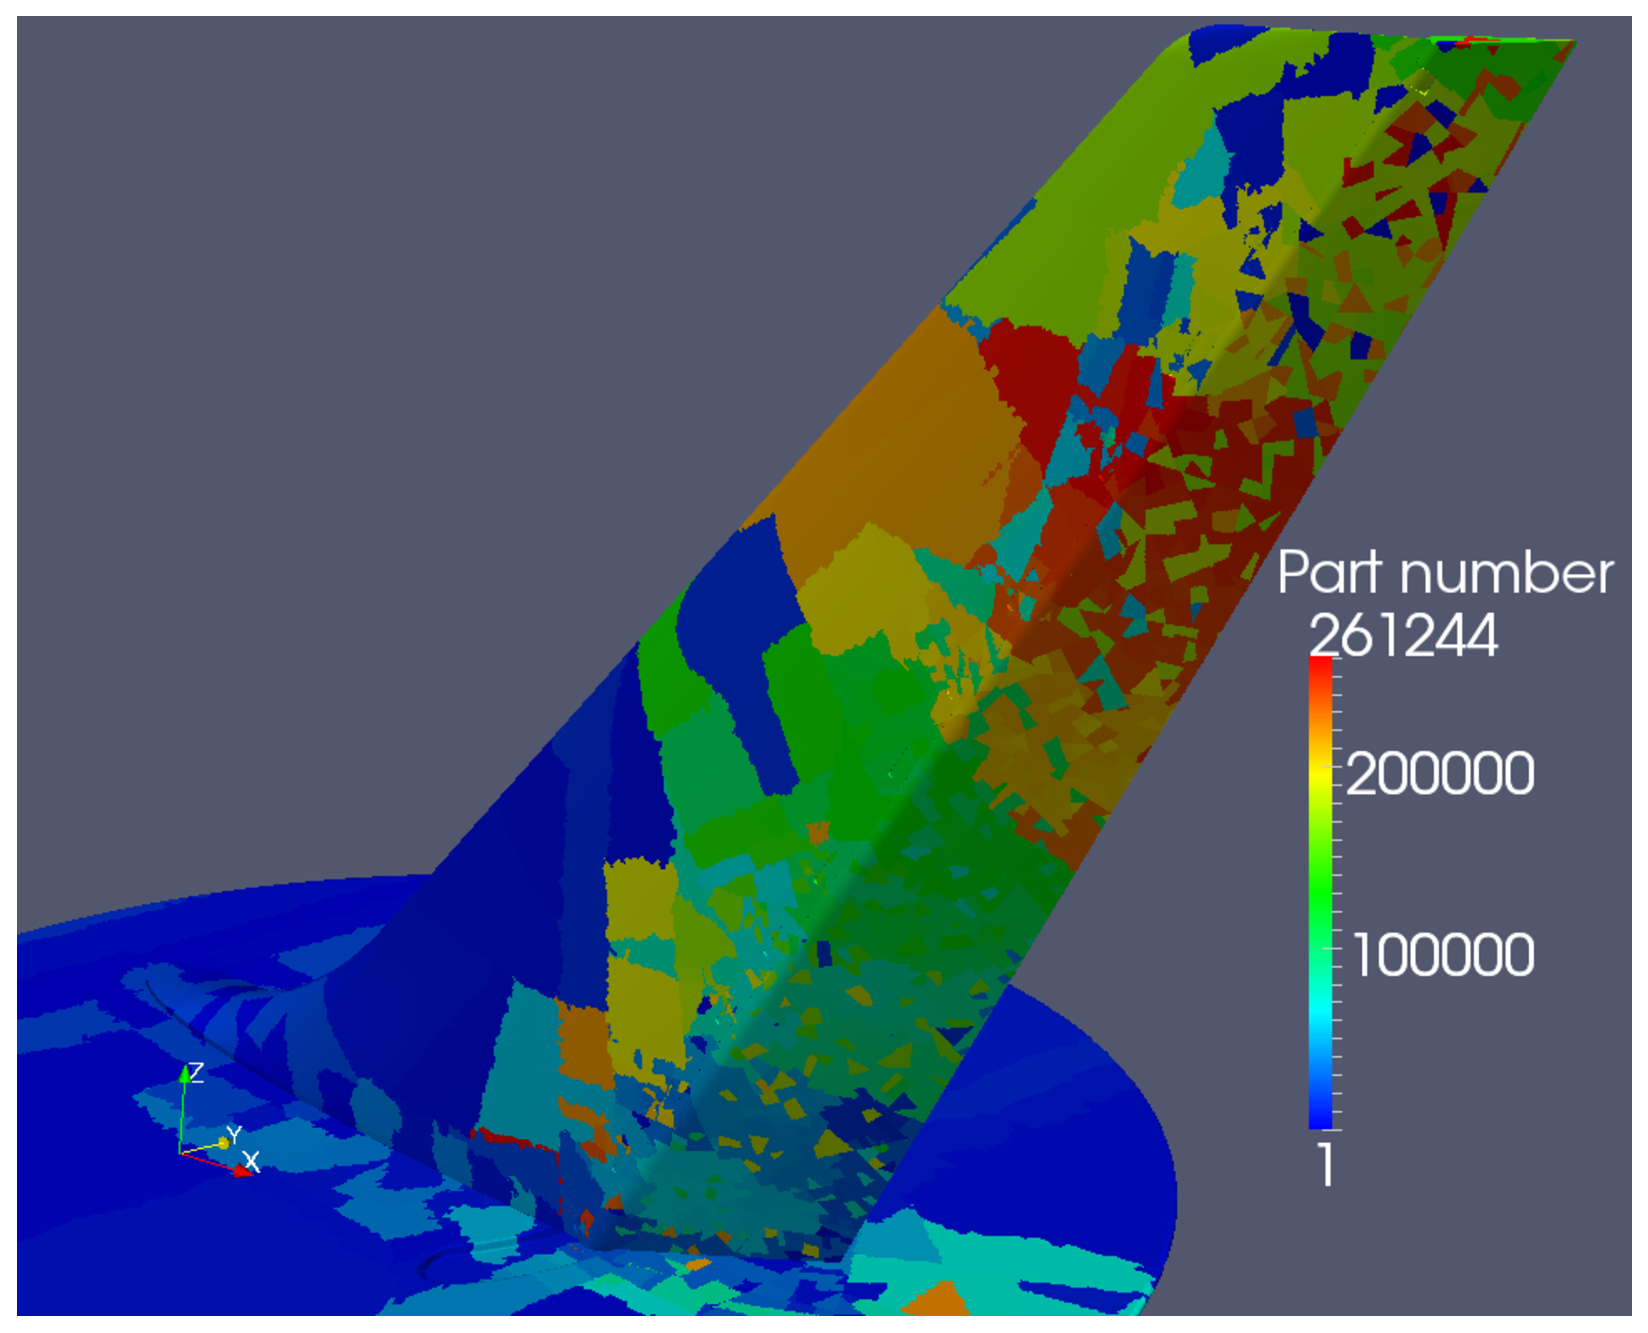
\includegraphics[width=.45\textwidth]{results/phasta/stabilizerFullView.eps}
  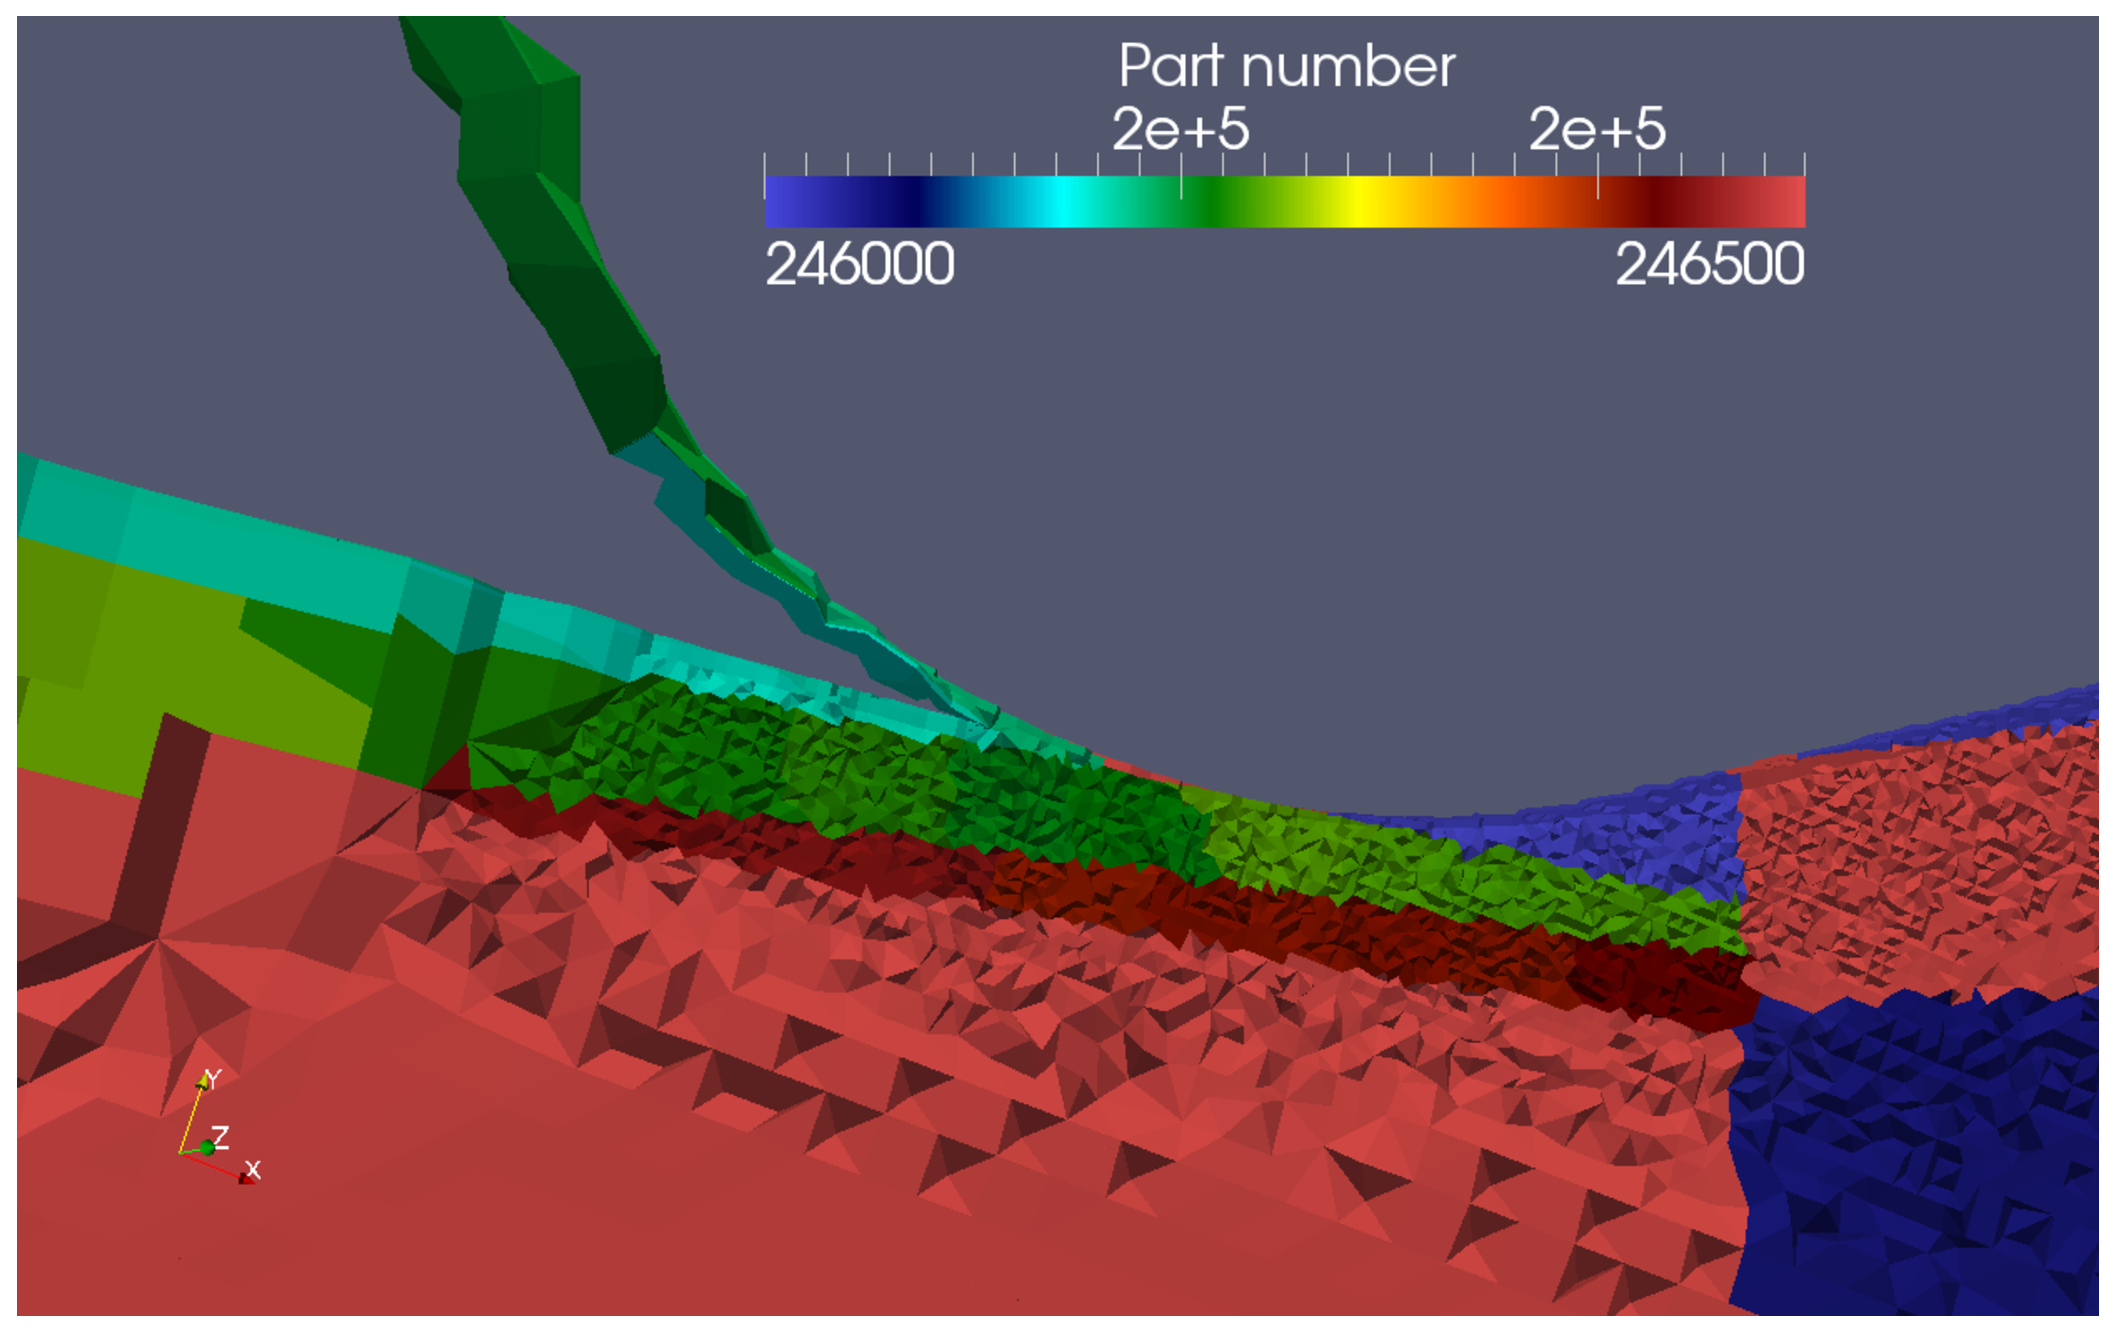
\includegraphics[width=.54\textwidth]{results/phasta/stabilizerGap.eps}
  \caption{
    (left) Full view of the vertical stabilizer and rudder and (right) a slice
    at their junction colored by part number illustrating the complex geometry
    and small features of the fluid mesh.
  }
  \label{fig:BoeingGeom}
\end{figure}

The flow in this case is solved by PHASTA.
PHASTA is a stabilized finite element analysis code~\cite{WhiJan01} using
an implicit solver.
The code is written in FORTRAN and is parallelized with MPI.
PHASTA's computational work is dominated by equation formation and equation solution.
Both types of work are executed on the same partition of mesh
elements~\cite{sahni2009scalable}.
An ideal partition will have balanced elements for equation formation work,
and balanced vertices, the degree-of-freedom holder, for equation solution work.
Furthermore, the partition will have parts with a low surface-to-volume ratio to
limit the cost of neighborhood communications that exchange information on
boundary vertices~\cite{rasquinCise2014}.

\begin{figure} \centering
  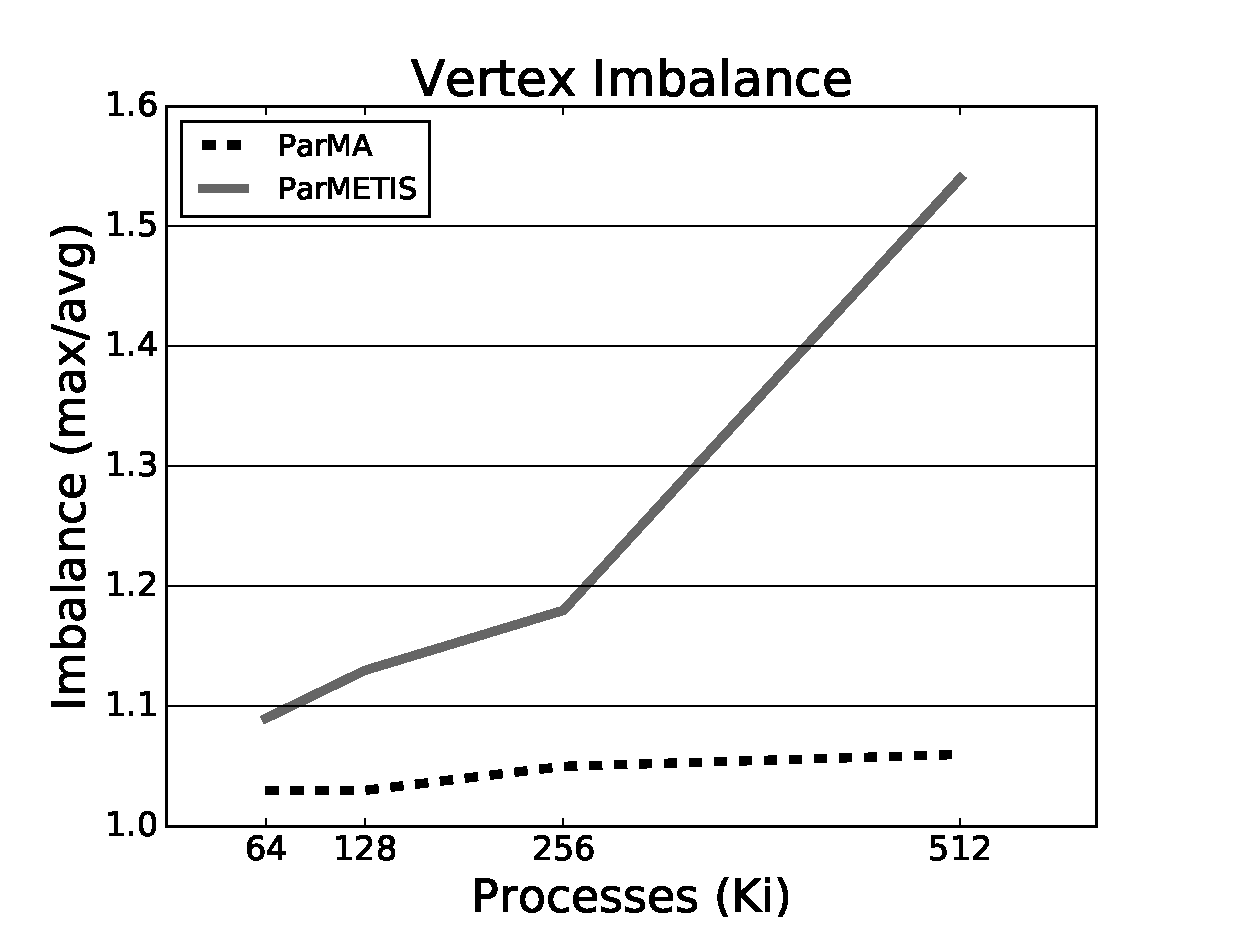
\includegraphics[width=.6\textwidth]{results/phasta/1B/vtxImb.eps}
  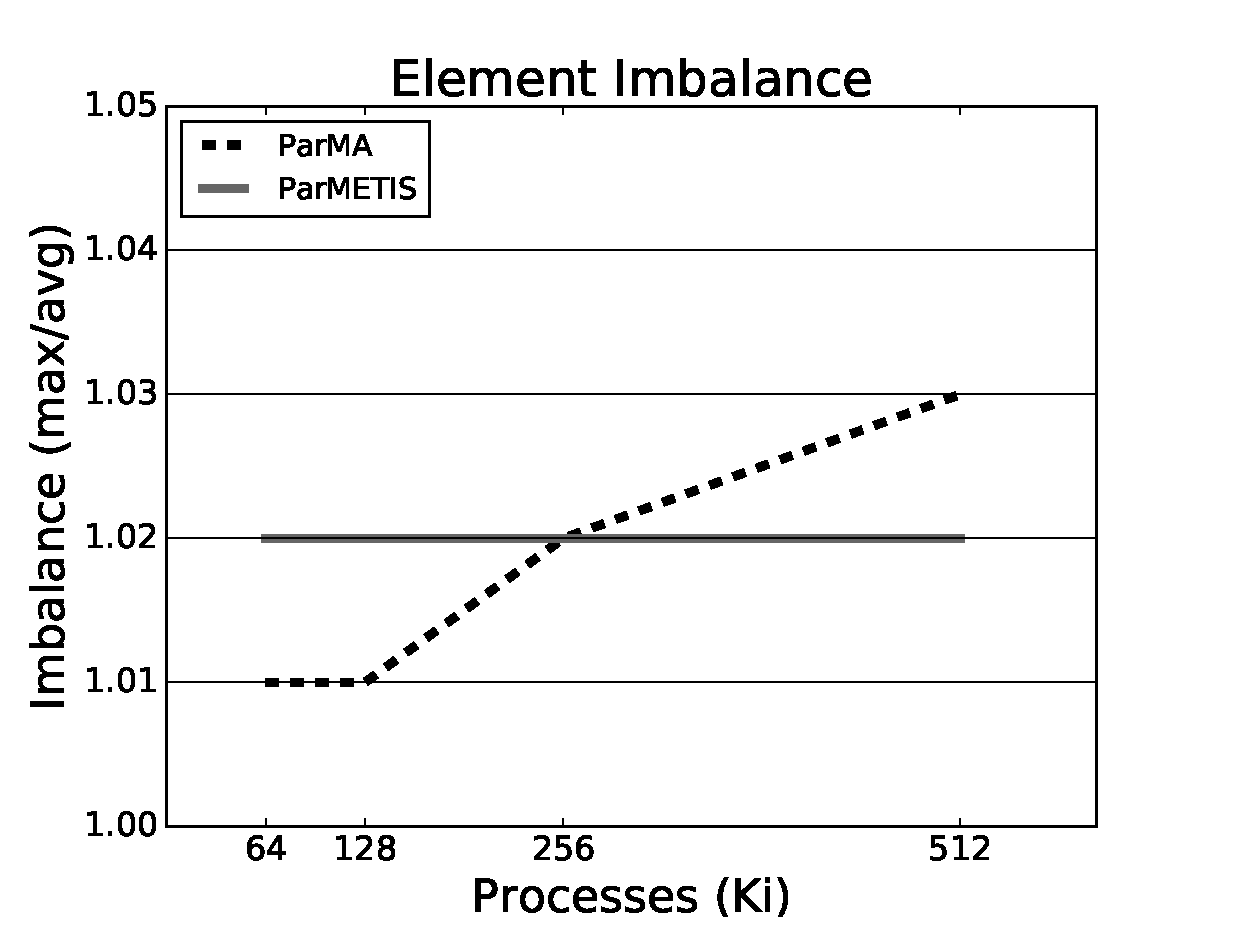
\includegraphics[width=.6\textwidth]{results/phasta/1B/elmImb.eps}
  \caption{Evolution of the (top) vertex and (bottom) element
    imbalance with and without ParMA.
  }
  \label{fig:ParmaBal}
\end{figure}

As shown in Fig.~\ref{fig:ParmaBal}, through three part-count doublings, ParMA is
able to improve the vertex imbalance with only insignificant increases in element
imbalance.
For example, in the largest partition, 512Ki parts, ParMA reduces the vertex 
imbalance from 54\% to 6\%, and only increases the element imbalance from 
1.8\% to 3\%.
As expected, the 1.2 percentage point increase in element imbalance has no effect 
on the nearly perfect scaling of equation formation (scaling factor of 0.96
maintained).
Critically though, ParMA improves the linear algebra work performance by 28\% over the
ParMETIS partition, and improves scaling from 0.82 to 1.14, as shown in
Fig.~\ref{fig:eqSolveImprovement}.
As sparse linear algebra is memory bandwidth limited~\cite{zhou2010adjacency}, a
super-linear scaling is observed as the working data size is reduced and cache
utilization is increased.
Similar, but less dramatic, performance and scaling gains are observed in the
256Ki part case.
In the smaller 64Ki and 128Ki partitions the performance difference is
negligible.

\begin{figure} \centering
  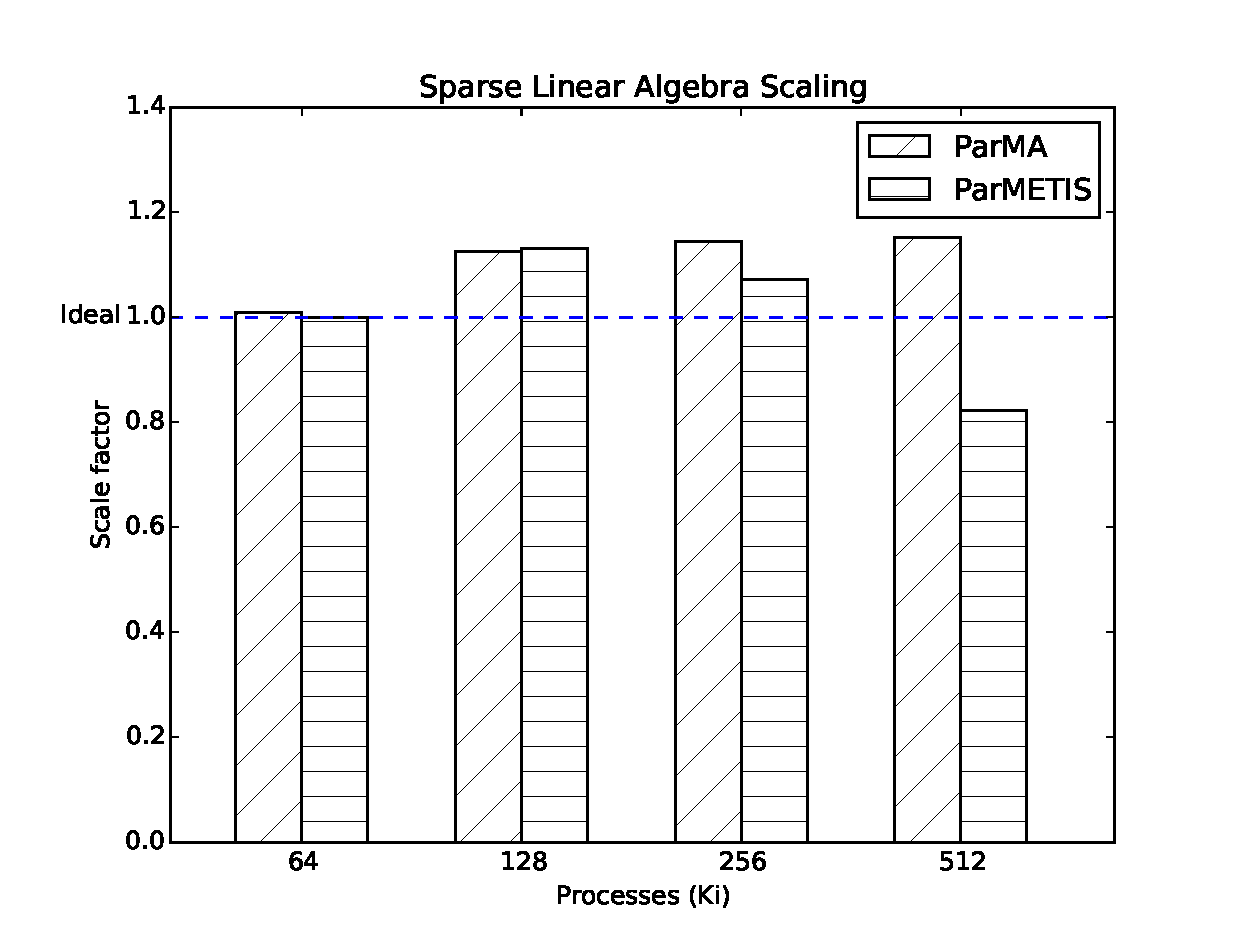
\includegraphics[width=.8\textwidth]{results/phasta/1B/linAlgWorkScaling.eps}
  \caption{Improvement of PHASTA sparse linear algebra scaling with ParMA.
           The PHASTA performance on the 64Ki ParMETIS partition
           is used as a baseline for all runs.
  }
  \label{fig:eqSolveImprovement}
\end{figure}
